\documentclass{article}
\pagestyle{empty}
\usepackage{graphicx}
\usepackage{hyperref}
\usepackage{listings}
\usepackage{subfigure}
\usepackage[margin=2.5cm]{geometry}
\setlength\parindent{0pt}
\usepackage{enumitem}
\usepackage{amsmath}
\usepackage{float}
\usepackage[extrafootnotefeatures]{xepersian}
\renewcommand{\labelitemi}{$\bullet$}
\settextfont[Scale=1]{B Zar}

\begin{document}
\begin{titlepage}
	\centering
	{\scshape\LARGE به نام خداوند بخشنده و مهربان \par}
	\vspace{2cm}
	{\huge\bfseries یادگیری عمیق\par}
	\vspace{3cm}
	{\Large\bfseries  پروژه درس \par}
	\vspace{3cm}
	{\Large\itshape 		محسن نقی‌پورفر		94106757\par}
	\vspace{0.25cm}
	\vfill
\end{titlepage}

\section{توضیح مختصری از کد}
در این قسمت یک توضیح مختصر از کد زده شده داده می‌شود. کد این پروژه به صورت ماژولار پیاده‌سازی شده است که یک پکیج را می‌سازد. این پکیچ به این صورت است از چند فایل کمکی مثل \lr{utils}، \lr{dataset} و ... کمک می‌گیرد. توابع کمکی در فایل \lr{utils} و تمام اعمال مورد نیاز برای دیتاست در فایل \lr{dataset} ذخیره شده است. همچنین در فایل‌‌های \lr{GAN}، \lr{CGAN} معماری های مورد نظر برای شبکه‌های مولد پیاده‌سازی شده  است. برای این پکیج از \lr{Tensorflow} استفاده شده است. همچنین کد موجود در فایل \lr{CNN}، یک شبکه کانوولوشنی عمیق برای دسته‌بندی استفاده شده است.
\subsection{توضیح فایل \lr{Dataset.py}}
در این فایل یک کلاس \lr{DataLoader}  پیاده‌سازی شده است که این کلاس برای اداره کردن همه توابع مختلف لازم برای داده‌های مورد نیاز برای شبکه‌های عصبی استفاده می‌شود.
\subsection{توضیح فایل \lr{GAN.py}}
در این فایل یک شبکه‌عصبی  \lr{GAN} به وسیله خود پکیج تنسورفلو پیاده‌سازی شده است. این شبکه در قالب یک کلاس پیاده‌سازی شده است.
\subsection{توضیح فایل \lr{CGAN.py}}
در این فایل، همانطور که از اسم آن نیز پیداست،‌ شبکه‌عصبی \lr{CGAN} به وسیله پکیج \lr{Keras} پیاده‌سازی شده است. این پیاده‌سازی به صورت شی‌گرا بوده است. همچنین همه توابع لازم برای رسم نمودار‌، کشیدن کاراکتر‌های جدید و ذخیره فایل لاگ حاصل از یادگیری این شبکه‌ نیز پیاده‌سازی شده است.
\subsection{توضیح فایل \lr{CNN.py}}
در این فایل شبکه کانولوشنی عمیق برای تشخیص نوع کاراکتر ورودی برای داده‌ حجیم داده 
شده استفاده شده است.
\section{توضیح معماری \lr{CNN}}
برای ساخت شبکه‌ \lr{CNN} برای دسته‌بندی حروف مختلف در بین فونت‌ها، از یک شبکه عصبی عمیقی استفاده شده است که دارای ۵ لایه کانوولوشن و \lr{Maxpooling} که به معماری آن به صورت زیر بوده است. شکل مربوط به معماری این شبکه‌ عصبی در زیر آمده است. برای عمیق‌تر کردن شبکه عصبی از ایده شبکه معروف \lr{VGG} استفاده شده است و از فیلتر های کوچک استفاده شده است تا شبکه عمیق‌تر شود البته در لایه از فیلتر ۱۱ در ۱۱ استفاده شده است. 

\begin{figure}[H]
	\centerline{\includegraphics[width=\textwidth , height=\textheight ]{CNN}}
	\caption{شبکه عصبی عمیق کانولوشنی استفاده شده در قسمت اول پروژه}
\end{figure}

\section{توضیح معماری \lr{Generator}}
برای شبکه \lr{Generator} موجود در معماری‌های \lr{CGAN} و \lr{GAN} از دو معماری مختلف استفاده‌ شده است. یکی شبکه‌ای کانولوشنی که از لایه \lr{Latent} (به همراه لایه \lr{Condition}  در شبکه \lr{CGAN}) و دیگری شبکه عصبی \lr{Fully Connected} خالص که هر دو آزمایش شده‌اند و نتایج حاصل از آن‌ها موجود می‌باشد. برای شبکه \lr{CGAN}،‌لایه \lr{Condition} به لایه \lr{Latent} چسبانده (\lr{Concatenate}) شده است. شکل مربوط به معماری شبکه‌ \lr{Generator} در زیر آمده است.
\begin{figure}[H]
	\centerline{\includegraphics[width=\textwidth , height=\textheight ]{G}}
	\caption{معماری شبکه \lr{Generator}}
\end{figure}

\section{توضیح معماری \lr{Discriminator}}
برای شبکه \lr{Discriminator} موجود در معماری‌های \lr{CGAN} و \lr{GAN} از دو معماری مختلف استفاده‌ شده است. یکی شبکه‌ای کانولوشنی که از لایه \lr{Image} (به همراه لایه \lr{Condition}  در شبکه \lr{CGAN}) و دیگری شبکه عصبی \lr{Fully Connected} خالص که هر دو آزمایش شده‌اند و نتایج حاصل از آن‌ها موجود می‌باشد. برای شبکه \lr{CGAN}،‌لایه \lr{Condition} در حالت \lr{FullyConnected} به لایه \lr{Image} چسبانده (\lr{Concatenate}) شده است. در واقع در این شبکه لایه \lr{Image} ابتدا \lr{Flat} شده است و یک لایه حاوی ۱۰۲۴ نورون را تشکیل داده است.شکل مربوط به معماری شبکه \lr{Discriminator} در زیر آمده است.
\begin{figure}[H]
	\centerline{\includegraphics[width=\textwidth , height=\textheight ]{D}}
	\caption{معماری شبکه \lr{Discriminator}}
\end{figure}
\begin{figure}[H]
	\centerline{\includegraphics[width=\textwidth , height=\textheight ]{CGAN}}
	\caption{معماری کلی شبکه \lr{CGAN} در زمان آموزش شبکه \lr{Generator}}
\end{figure}
\section{توضیح نحوه آموزش شبکه‌های مولد}
برای آموزش ‌شبکه‌های مولد، از \lr{Trick}‌های مختلفی استفاده شده است. این تریک‌ها در زیر آورده شده‌اند.  
\begin{itemize}
	\item استفاده از الگوریتم بهینه‌سازی \lr{Adam} برای شبکه \lr{Generator} و الگوریتم بهینه‌سازی \lr{SGD} برای شبکه \lr{Discriminator}
	\item استفاده از تکنیک \lr{Label Smoothing} برای آموزش هر دو شبکه \lr{Generator} و \lr{Discriminator}
	\item استفاده از تابع فعال‌ساز \lr{LeakyReLU} با پارامتر ۰.۲ بعد از هر لایه در معماری شبکه‌های \lr{Generator} و \lr{Discriminator}
	\item آموزش جدای داده‌های \lr{real}و \lr{fake} به شبکه \lr{Discriminator} به جای آموزش ترکیبی از آنها (\lr{concatenation}ای از آنها)
	\item نرمالیزه کردن دیتای ورودی برای آموزش شبکه‌های مولد(نگاشت بازه هر پیکسل  ورودی به ۱ و ۱-)
	\item آموزش داده‌های واقعی با برچسب صفر و داده‌های غیر واقعی با برچسب ۱ برای شبکه \lr{Generator} 
\end{itemize}

\section{نتایج بدست آمده در قسمت اول}
برای شبکه اول، از تمام داده‌های \lr{Training} برای آموزش استفاده شده است و از داده \lr{X\_test} داده شده برای داده \lr{Validation} و ارزیابی شبکه‌ استفاده شده است. نمودار یادگیری برای داده آموزش و تست برای این شبکه در زیر آمده است.
\section{نتایج بدست آمده در قسمت دوم}
برای این قسمت نتایج عظیمی فراهم شده است! اکثر این نتایج در پوشه‌ \lr{results} ضمیمه شده‌اند. همچنین عکس‌های مربوط به تولید جمله مورد نظر در صورت پروژه و کاراکتر‌های مختلف در طول آموزش شبکه \lr{CGAN} در زیر آمده است.
\subsection{حروف الفبا}
\begin{figure}[H]
	\centerline{\includegraphics[width=\textwidth , height=\textheight ]{../results/CGAN_Adam/figs/Alphabet_(Epoch=75)}}
	\caption{عکس‌های الفبای یادگرفته شده در ایپاک ۷۵ام در شبکه عصبی}
\end{figure}
\begin{figure}[H]
	\centerline{\includegraphics[width=\textwidth , height=\textheight ]{../results/CGAN_Adam/figs/Alphabet_(Epoch=80)}}
	\caption{عکس‌های الفبای یادگرفته شده در ایپاک ۸۰ام در شبکه عصبی}
\end{figure}
\begin{figure}[H]
	\centerline{\includegraphics[width=\textwidth , height=\textheight ]{../results/CGAN_Adam/figs/Alphabet_(Epoch=85)}}
	\caption{عکس‌های الفبای یادگرفته شده در ایپاک ۸۵ام در شبکه عصبی}
\end{figure}
\begin{figure}[H]
	\centerline{\includegraphics[width=\textwidth , height=\textheight ]{../results/CGAN_Adam/figs/Alphabet_(Epoch=90)}}
	\caption{عکس‌های الفبای یادگرفته شده در ایپاک ۹۰ام در شبکه عصبی}
\end{figure}
\begin{figure}[H]
	\centerline{\includegraphics[width=\textwidth , height=\textheight ]{../results/CGAN_Adam/figs/Alphabet_(Epoch=95)}}
	\caption{عکس‌های الفبای یادگرفته شده در ایپاک ۹۵ام در شبکه عصبی}
\end{figure}

% ----------------------------------------------------------------------
\subsection{حرف \lr{A}}
\begin{figure}[H]
	\centerline{\includegraphics[width=\textwidth , height=\textheight ]{../results/CGAN_Adam/figs/letters/A/95.pdf}}
\end{figure}
\begin{figure}[H]
	\centerline{\includegraphics[width=\textwidth , height=\textheight ]{../results/CGAN_Adam/figs/letters/A/90.pdf}}
\end{figure}

\subsection{حرف \lr{B}}
\begin{figure}[H]
	\centerline{\includegraphics[width=\textwidth , height=\textheight ]{../results/CGAN_Adam/figs/letters/B/95.pdf}}
\end{figure}
\begin{figure}[H]
	\centerline{\includegraphics[width=\textwidth , height=\textheight ]{../results/CGAN_Adam/figs/letters/B/90.pdf}}
\end{figure}

\subsection{حرف \lr{C}}
\begin{figure}[H]
	\centerline{\includegraphics[width=\textwidth , height=\textheight ]{../results/CGAN_Adam/figs/letters/C/95.pdf}}
\end{figure}
\begin{figure}[H]
	\centerline{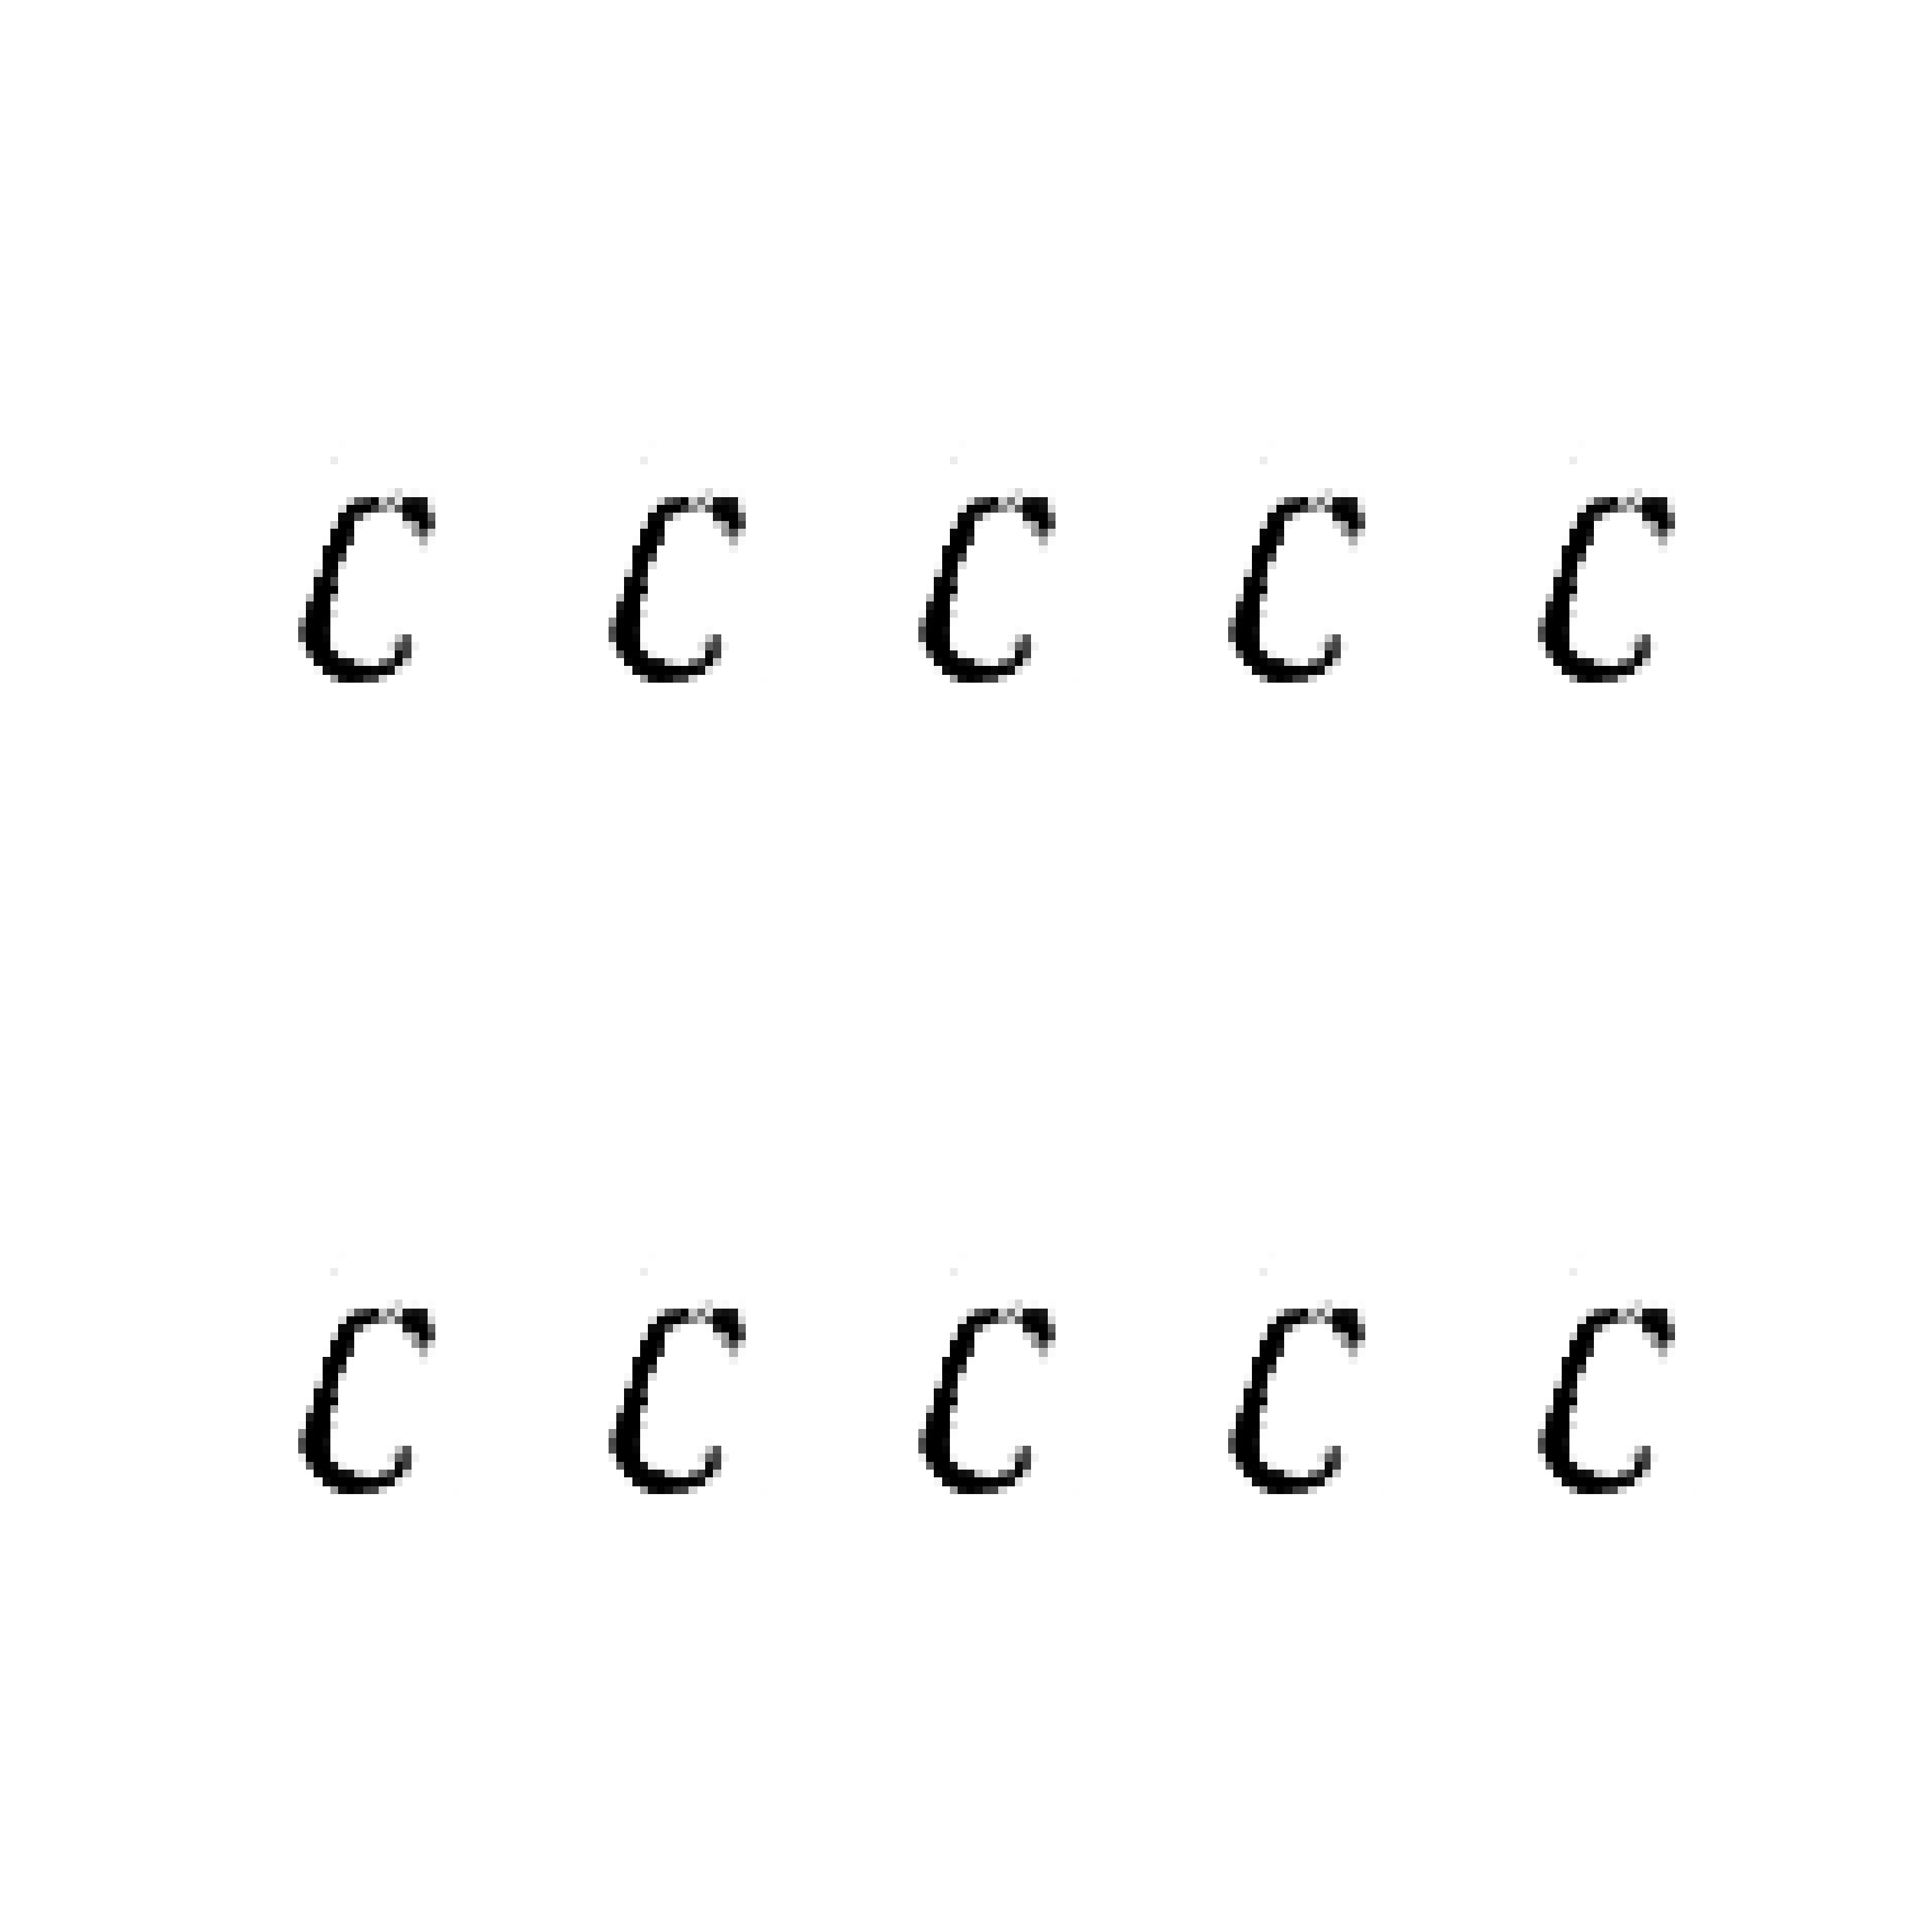
\includegraphics[width=\textwidth , height=\textheight ]{../results/CGAN_Adam/figs/letters/C/90.pdf}}
\end{figure}

\subsection{حرف \lr{D}}
\begin{figure}[H]
	\centerline{\includegraphics[width=\textwidth , height=\textheight ]{../results/CGAN_Adam/figs/letters/D/95.pdf}}
\end{figure}
\begin{figure}[H]
	\centerline{\includegraphics[width=\textwidth , height=\textheight ]{../results/CGAN_Adam/figs/letters/D/90.pdf}}
\end{figure}

\subsection{حرف \lr{E}}
\begin{figure}[H]
	\centerline{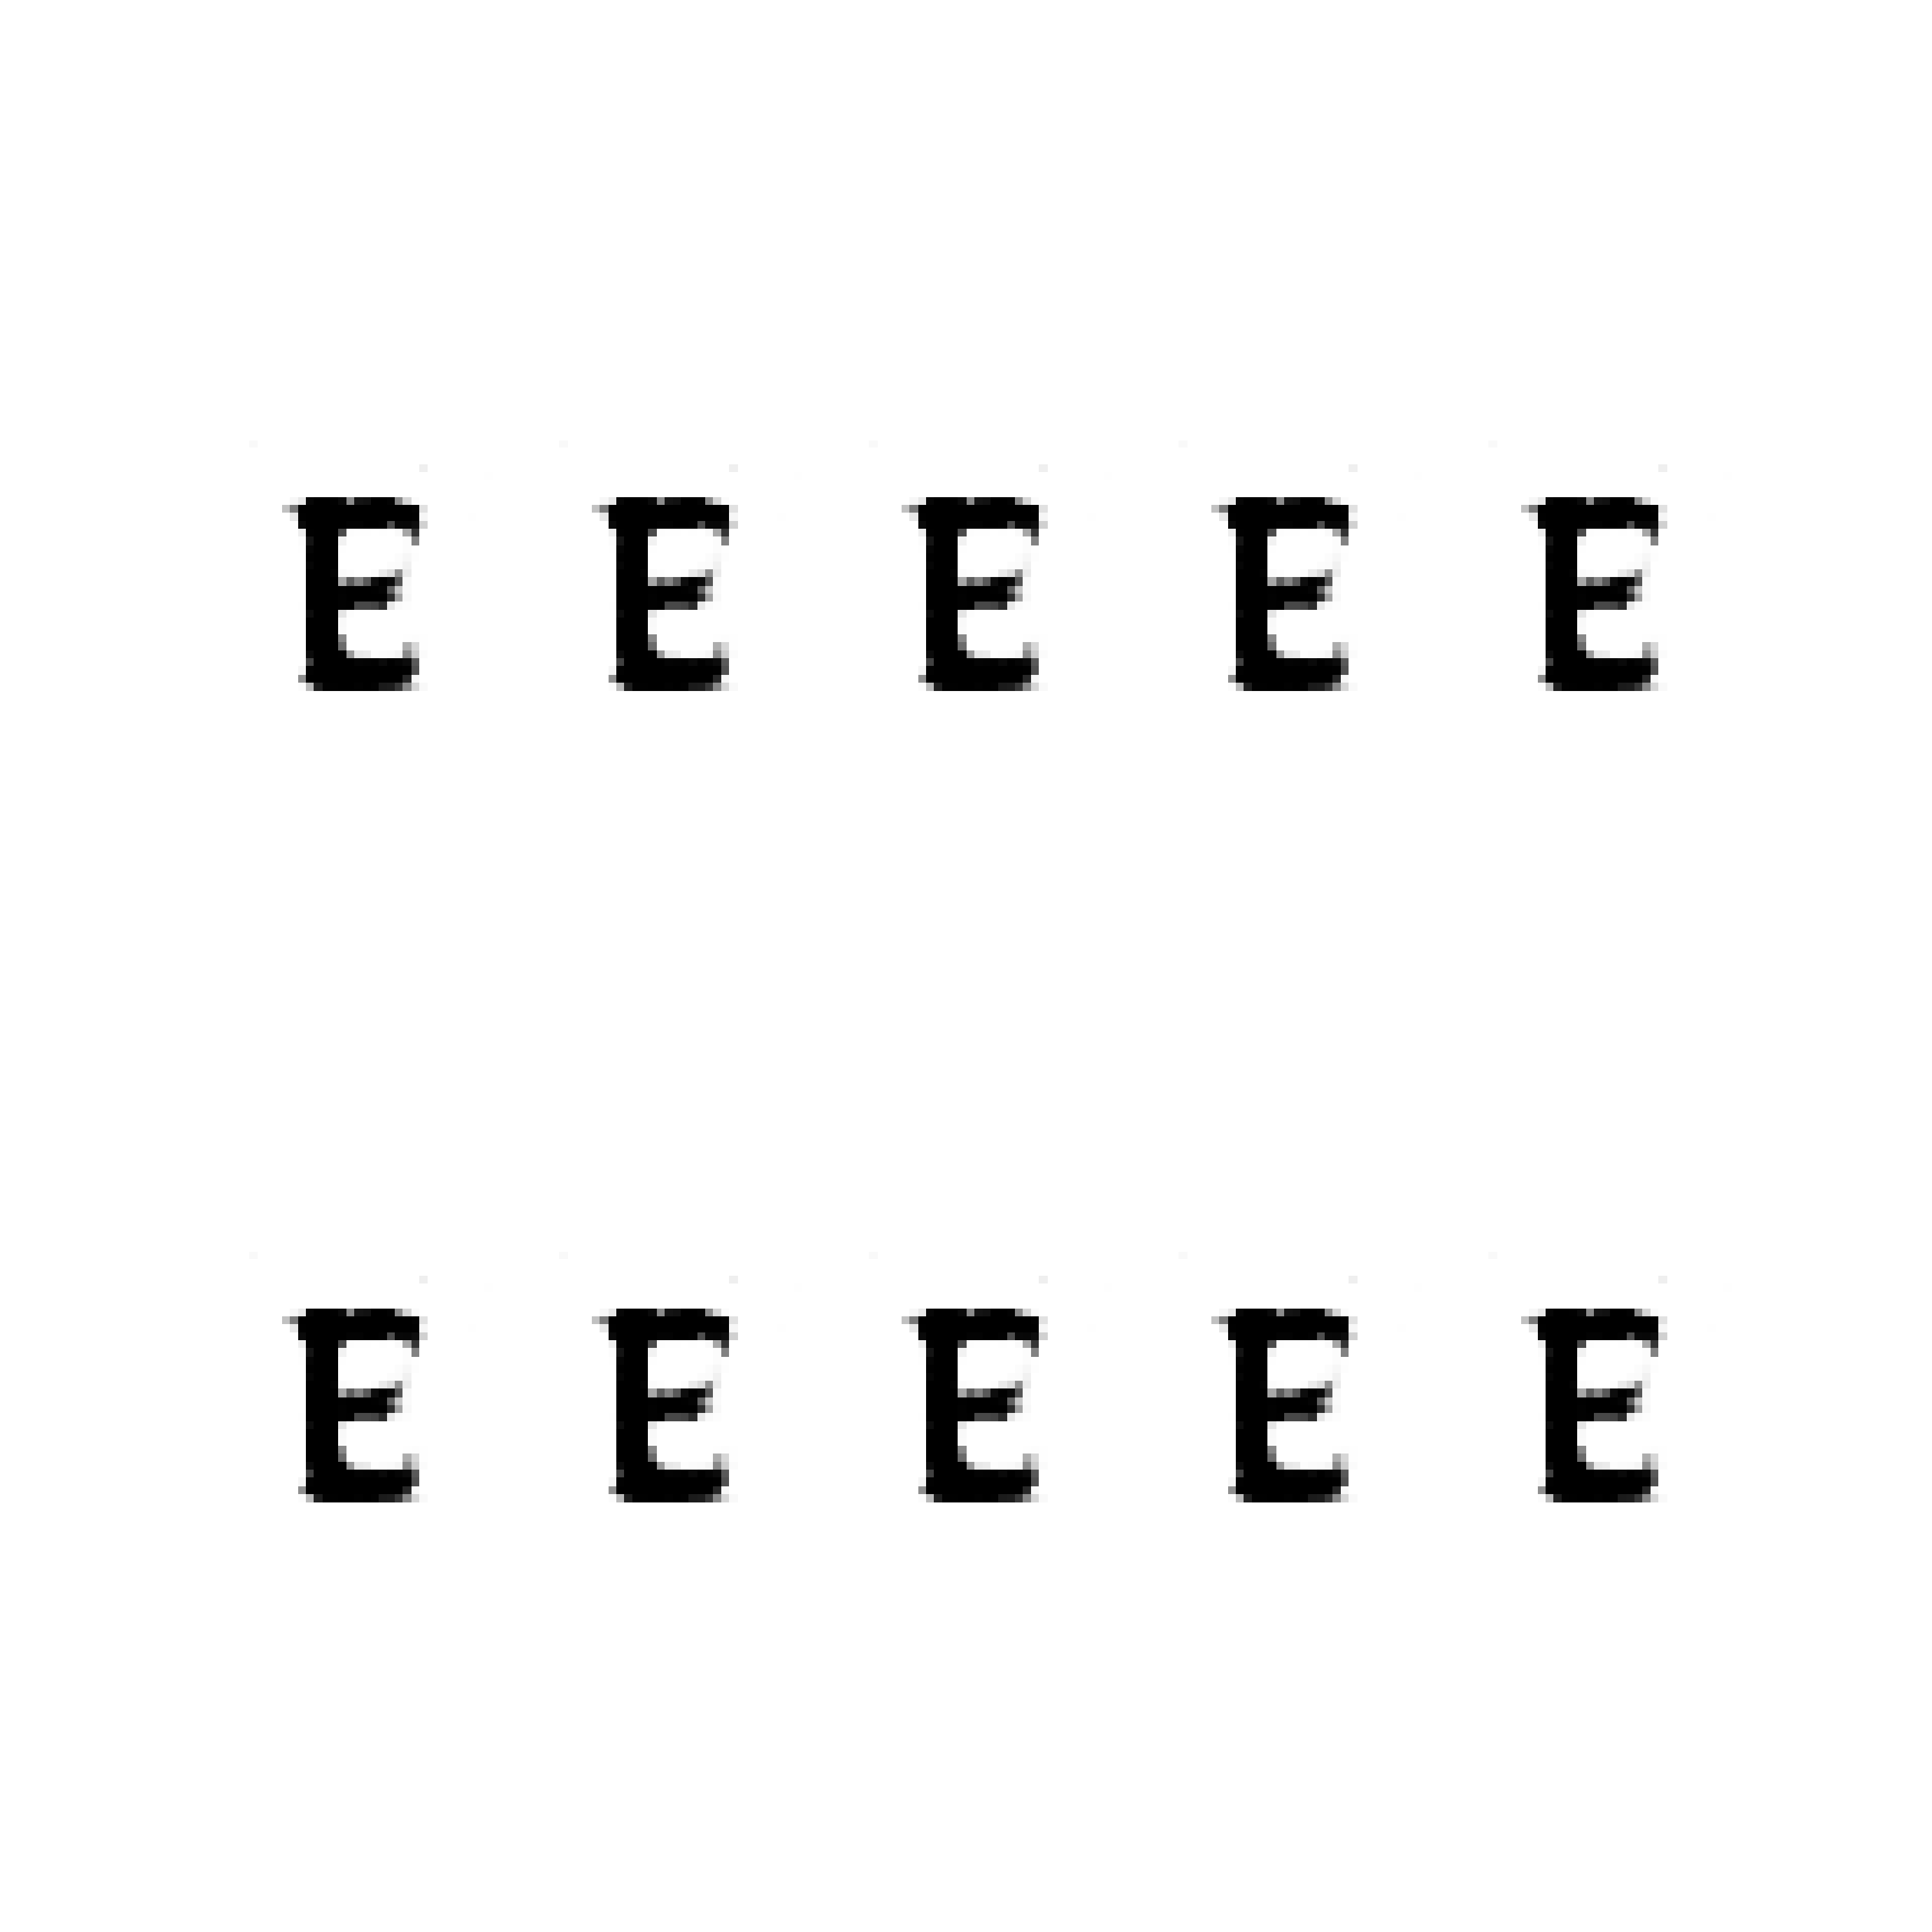
\includegraphics[width=\textwidth , height=\textheight ]{../results/CGAN_Adam/figs/letters/E/95.pdf}}
\end{figure}
\begin{figure}[H]
	\centerline{\includegraphics[width=\textwidth , height=\textheight ]{../results/CGAN_Adam/figs/letters/E/90.pdf}}
\end{figure}

\subsection{حرف \lr{F}}
\begin{figure}[H]
	\centerline{\includegraphics[width=\textwidth , height=\textheight ]{../results/CGAN_Adam/figs/letters/F/95.pdf}}
\end{figure}
\begin{figure}[H]
	\centerline{\includegraphics[width=\textwidth , height=\textheight ]{../results/CGAN_Adam/figs/letters/F/90.pdf}}
\end{figure}

\subsection{حرف \lr{G}}
\begin{figure}[H]
	\centerline{\includegraphics[width=\textwidth , height=\textheight ]{../results/CGAN_Adam/figs/letters/G/95.pdf}}
\end{figure}
\begin{figure}[H]
	\centerline{\includegraphics[width=\textwidth , height=\textheight ]{../results/CGAN_Adam/figs/letters/G/90.pdf}}
\end{figure}

\subsection{حرف \lr{H}}
\begin{figure}[H]
	\centerline{\includegraphics[width=\textwidth , height=\textheight ]{../results/CGAN_Adam/figs/letters/H/95.pdf}}
\end{figure}
\begin{figure}[H]
	\centerline{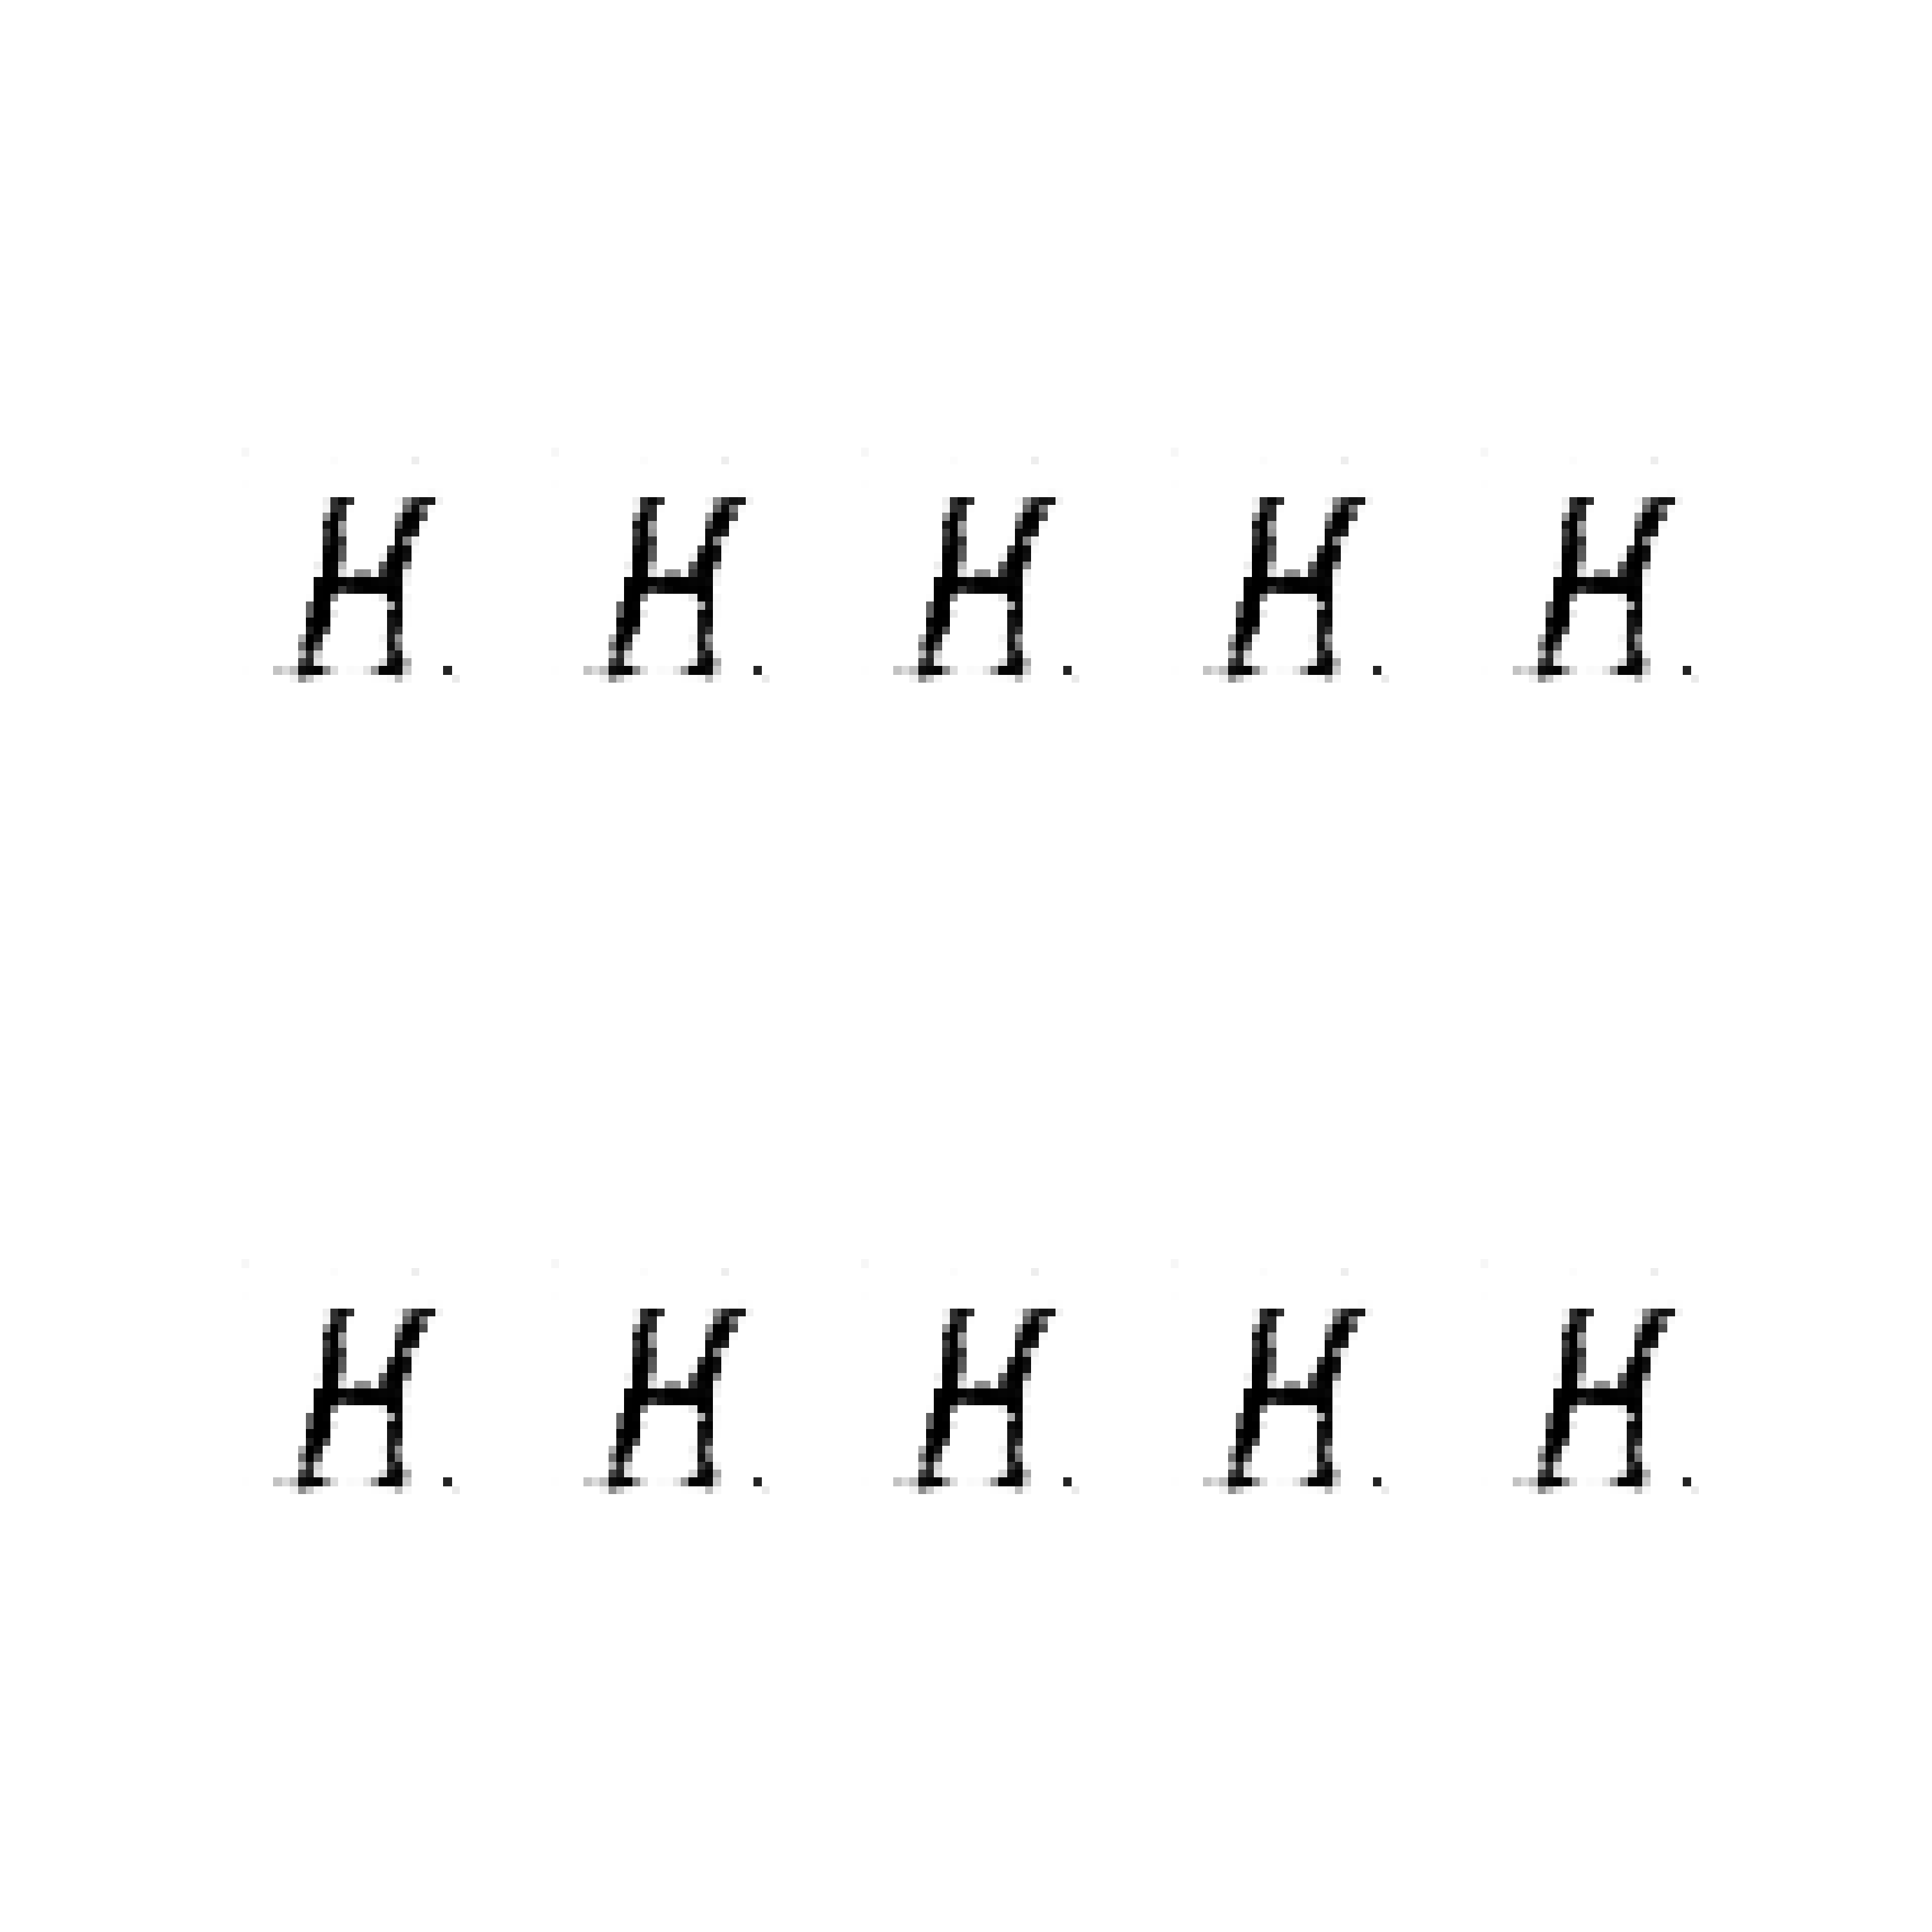
\includegraphics[width=\textwidth , height=\textheight ]{../results/CGAN_Adam/figs/letters/H/90.pdf}}
\end{figure}

\subsection{حرف \lr{I}}
\begin{figure}[H]
	\centerline{\includegraphics[width=\textwidth , height=\textheight ]{../results/CGAN_Adam/figs/letters/I/95.pdf}}
\end{figure}
\begin{figure}[H]
	\centerline{\includegraphics[width=\textwidth , height=\textheight ]{../results/CGAN_Adam/figs/letters/I/90.pdf}}
\end{figure}

\subsection{حرف \lr{J}}
\begin{figure}[H]
	\centerline{\includegraphics[width=\textwidth , height=\textheight ]{../results/CGAN_Adam/figs/letters/J/95.pdf}}
\end{figure}
\begin{figure}[H]
	\centerline{\includegraphics[width=\textwidth , height=\textheight ]{../results/CGAN_Adam/figs/letters/J/90.pdf}}
\end{figure}

\subsection{حرف \lr{K}}
\begin{figure}[H]
	\centerline{\includegraphics[width=\textwidth , height=\textheight ]{../results/CGAN_Adam/figs/letters/K/95.pdf}}
\end{figure}
\begin{figure}[H]
	\centerline{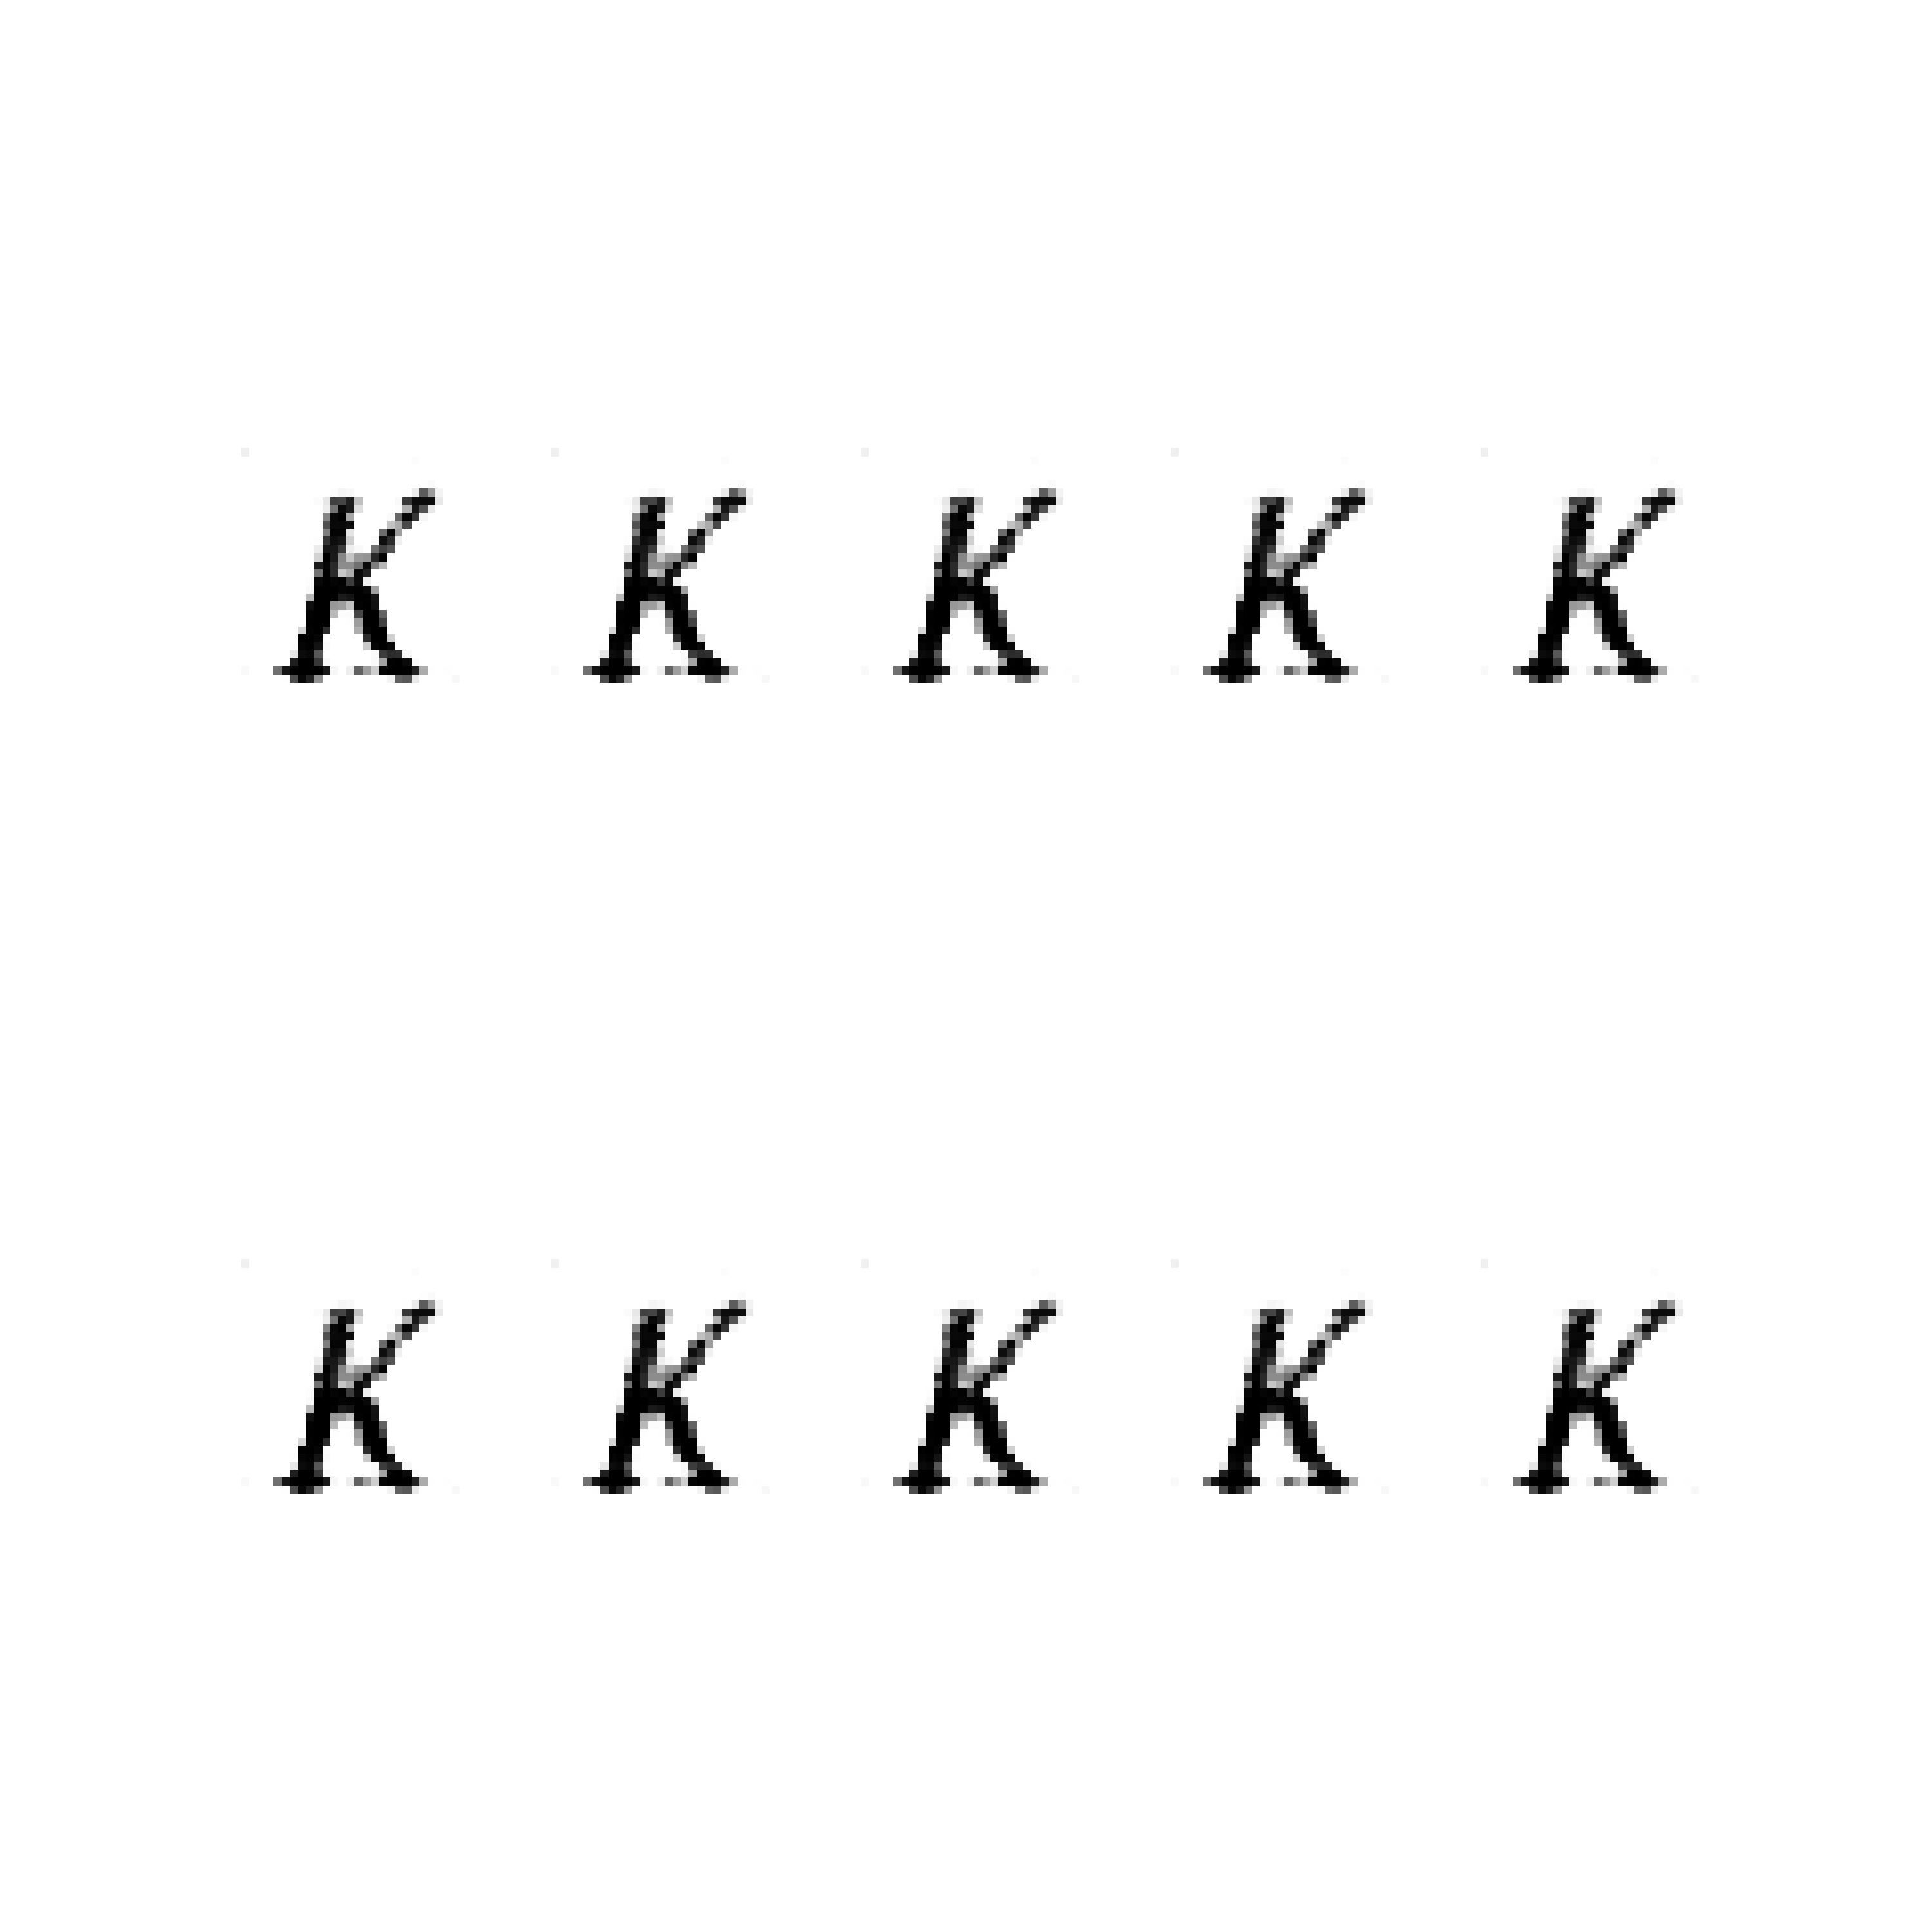
\includegraphics[width=\textwidth , height=\textheight ]{../results/CGAN_Adam/figs/letters/K/90.pdf}}
\end{figure}

\subsection{حرف \lr{L}}
\begin{figure}[H]
	\centerline{\includegraphics[width=\textwidth , height=\textheight ]{../results/CGAN_Adam/figs/letters/L/95.pdf}}
\end{figure}
\begin{figure}[H]
	\centerline{\includegraphics[width=\textwidth , height=\textheight ]{../results/CGAN_Adam/figs/letters/L/90.pdf}}
\end{figure}

\subsection{حرف \lr{M}}
\begin{figure}[H]
	\centerline{\includegraphics[width=\textwidth , height=\textheight ]{../results/CGAN_Adam/figs/letters/M/95.pdf}}
\end{figure}
\begin{figure}[H]
	\centerline{\includegraphics[width=\textwidth , height=\textheight ]{../results/CGAN_Adam/figs/letters/M/90.pdf}}
\end{figure}

\subsection{حرف \lr{N}}
\begin{figure}[H]
	\centerline{\includegraphics[width=\textwidth , height=\textheight ]{../results/CGAN_Adam/figs/letters/N/95.pdf}}
\end{figure}
\begin{figure}[H]
	\centerline{\includegraphics[width=\textwidth , height=\textheight ]{../results/CGAN_Adam/figs/letters/N/90.pdf}}
\end{figure}

\subsection{حرف \lr{O}}
\begin{figure}[H]
	\centerline{\includegraphics[width=\textwidth , height=\textheight ]{../results/CGAN_Adam/figs/letters/O/95.pdf}}
\end{figure}
\begin{figure}[H]
	\centerline{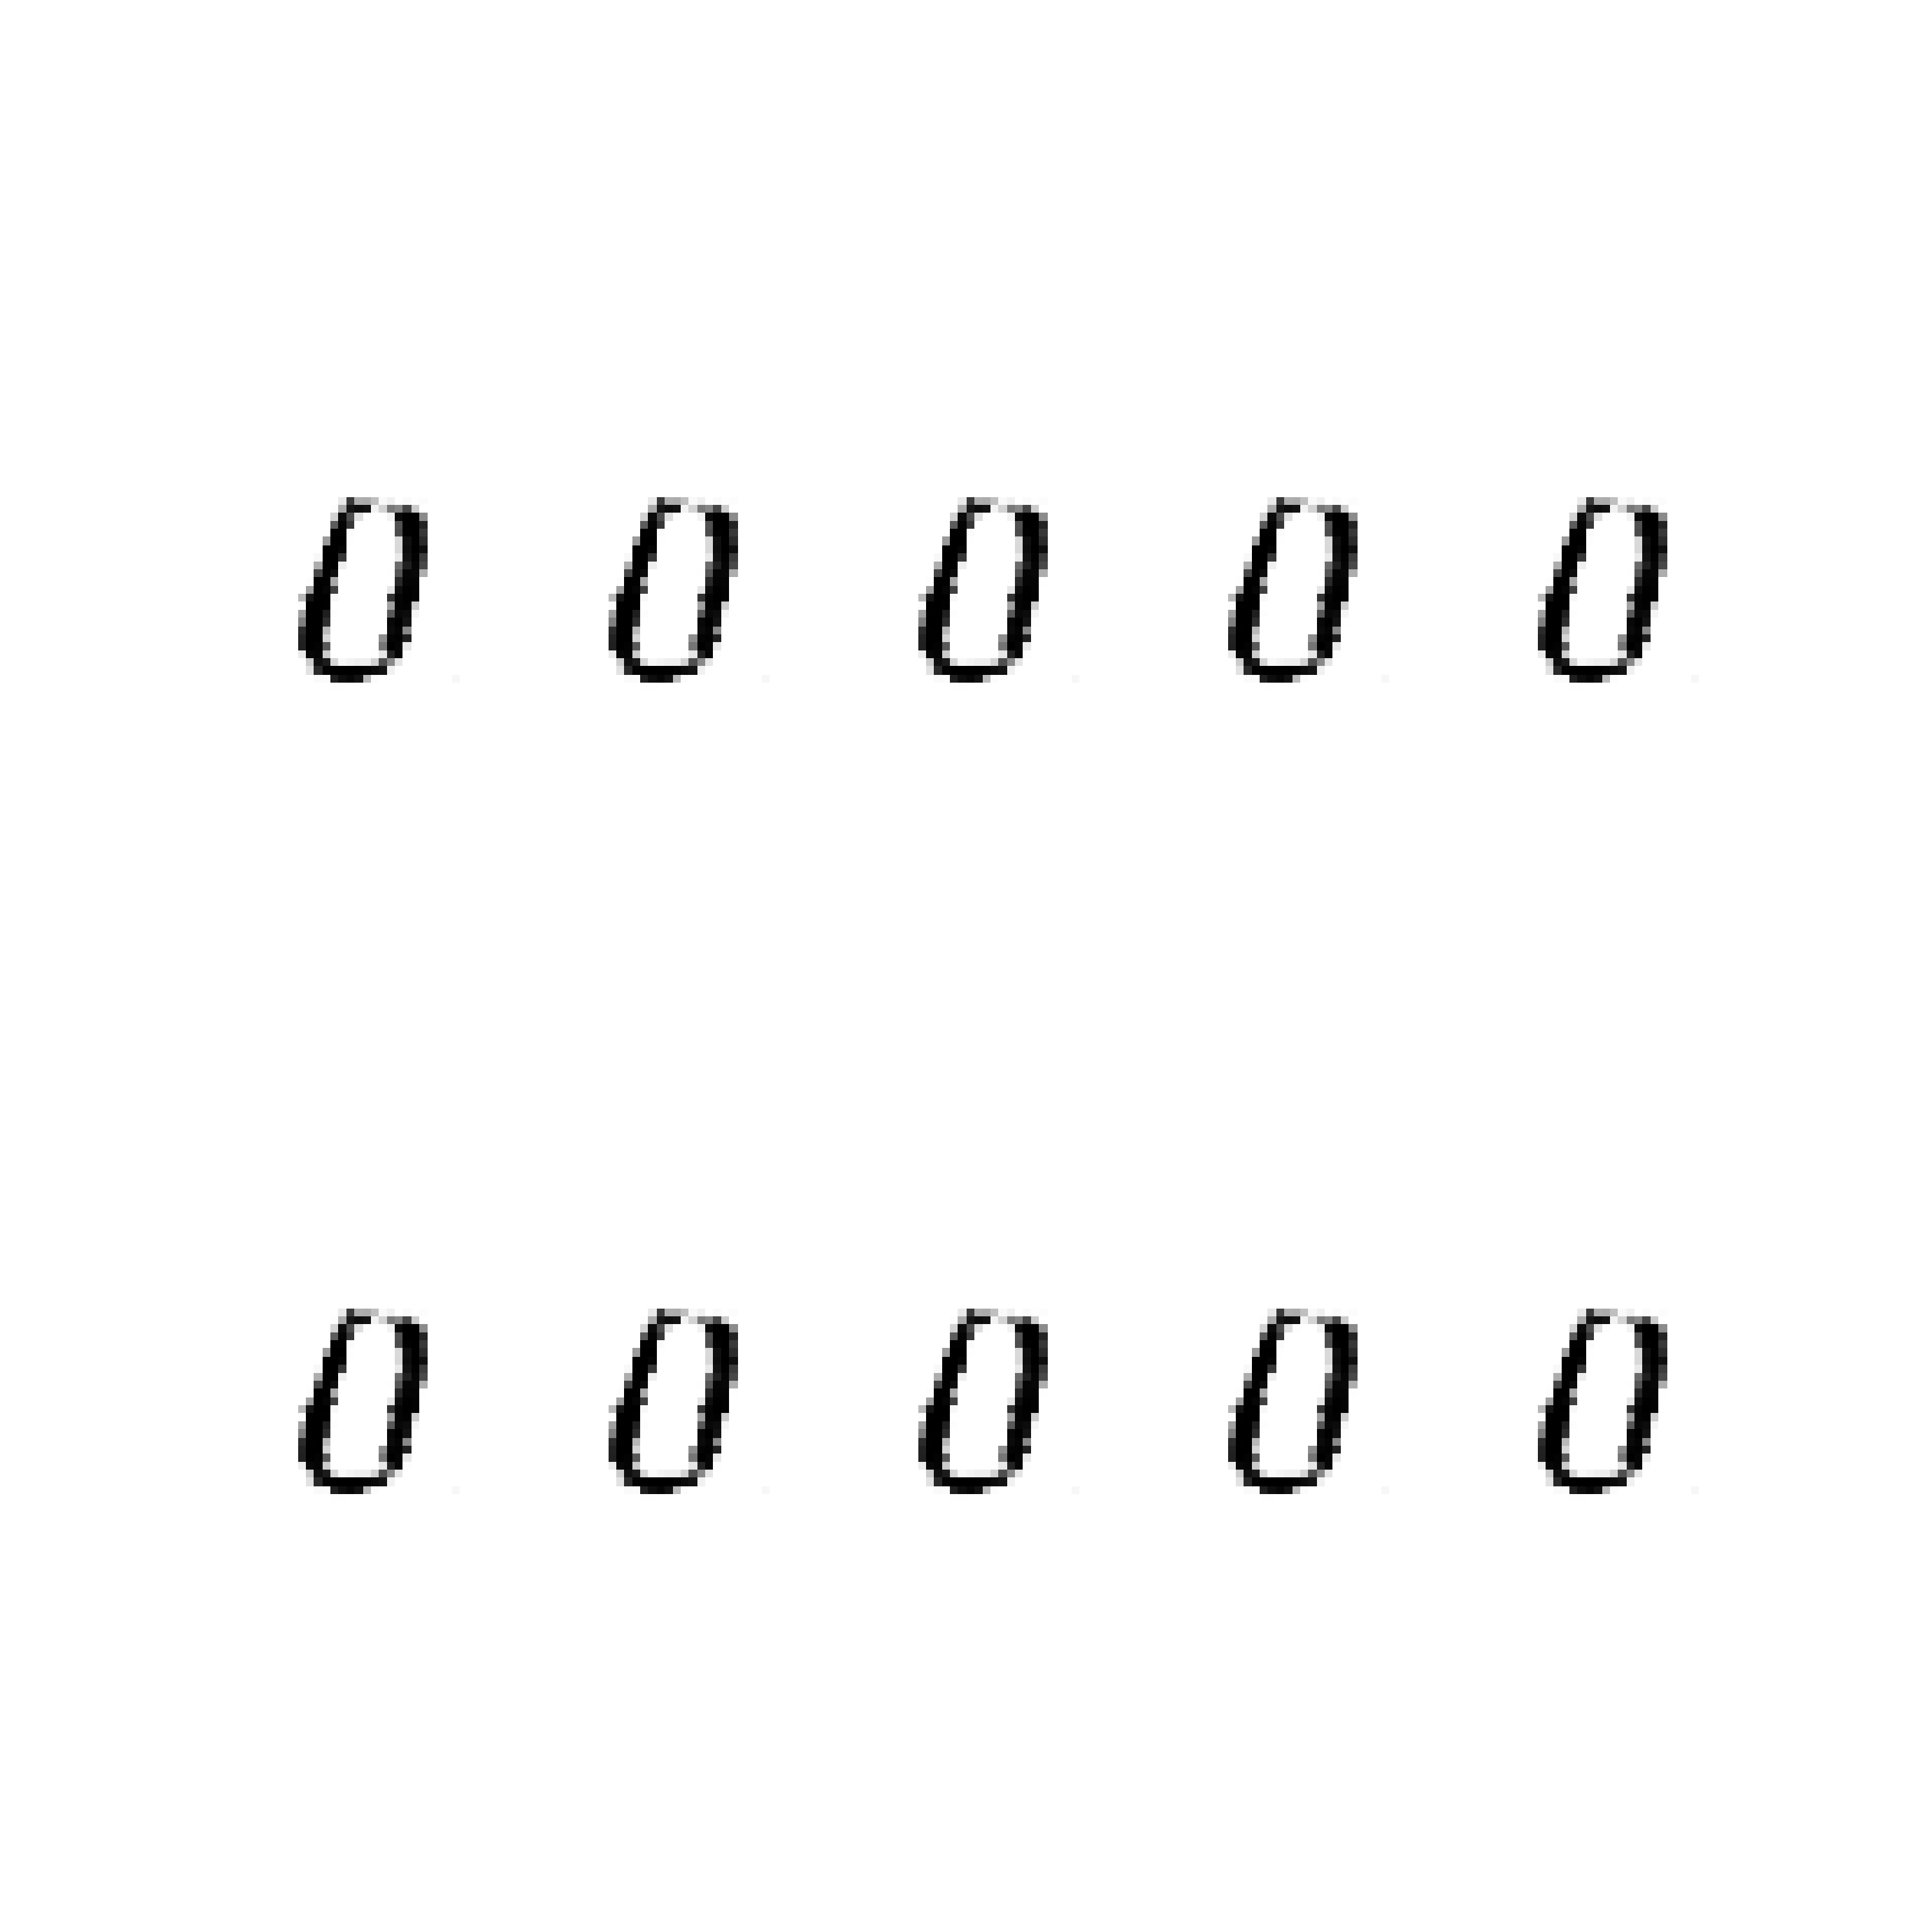
\includegraphics[width=\textwidth , height=\textheight ]{../results/CGAN_Adam/figs/letters/O/90.pdf}}
\end{figure}

\subsection{حرف \lr{P}}
\begin{figure}[H]
	\centerline{\includegraphics[width=\textwidth , height=\textheight ]{../results/CGAN_Adam/figs/letters/P/95.pdf}}
\end{figure}
\begin{figure}[H]
	\centerline{\includegraphics[width=\textwidth , height=\textheight ]{../results/CGAN_Adam/figs/letters/P/90.pdf}}
\end{figure}

\subsection{حرف \lr{Q}}
\begin{figure}[H]
	\centerline{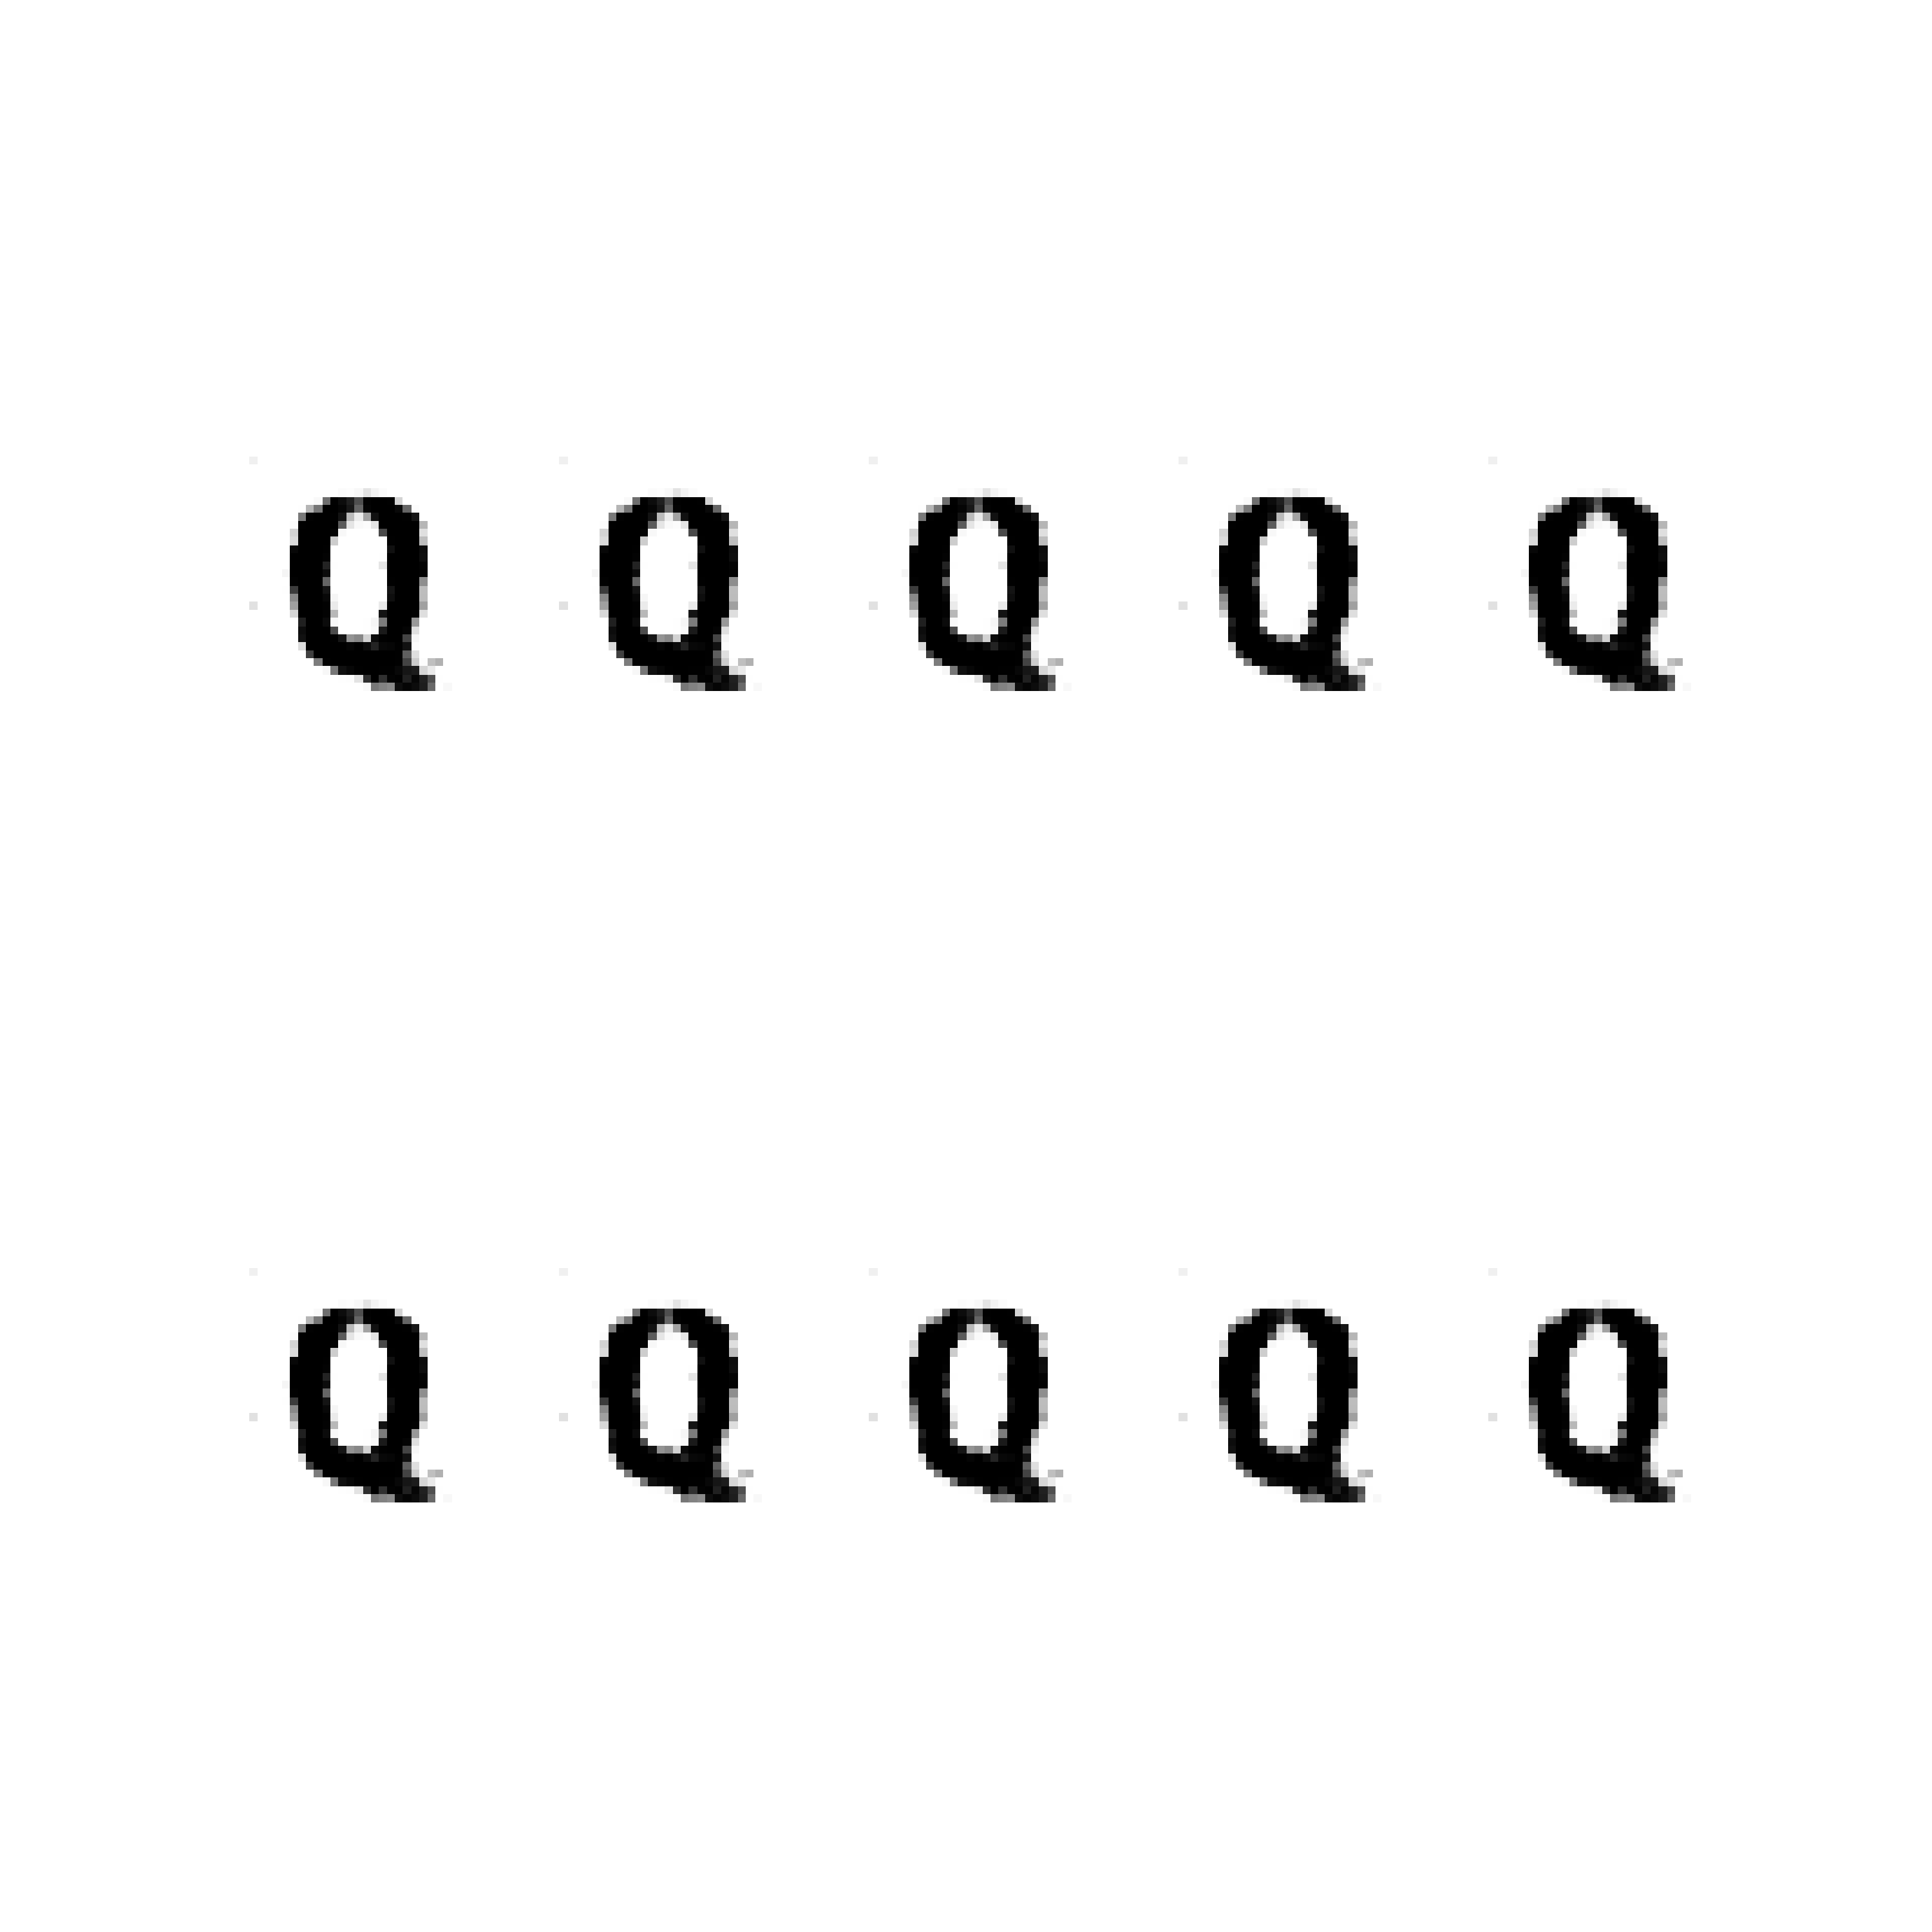
\includegraphics[width=\textwidth , height=\textheight ]{../results/CGAN_Adam/figs/letters/Q/95.pdf}}
\end{figure}
\begin{figure}[H]
	\centerline{\includegraphics[width=\textwidth , height=\textheight ]{../results/CGAN_Adam/figs/letters/Q/90.pdf}}
\end{figure}

\subsection{حرف \lr{R}}
\begin{figure}[H]
	\centerline{\includegraphics[width=\textwidth , height=\textheight ]{../results/CGAN_Adam/figs/letters/R/95.pdf}}
\end{figure}
\begin{figure}[H]
	\centerline{\includegraphics[width=\textwidth , height=\textheight ]{../results/CGAN_Adam/figs/letters/R/90.pdf}}
\end{figure}

\subsection{حرف \lr{S}}
\begin{figure}[H]
	\centerline{\includegraphics[width=\textwidth , height=\textheight ]{../results/CGAN_Adam/figs/letters/S/95.pdf}}
\end{figure}
\begin{figure}[H]
	\centerline{\includegraphics[width=\textwidth , height=\textheight ]{../results/CGAN_Adam/figs/letters/S/90.pdf}}
\end{figure}

\subsection{حرف \lr{T}}
\begin{figure}[H]
	\centerline{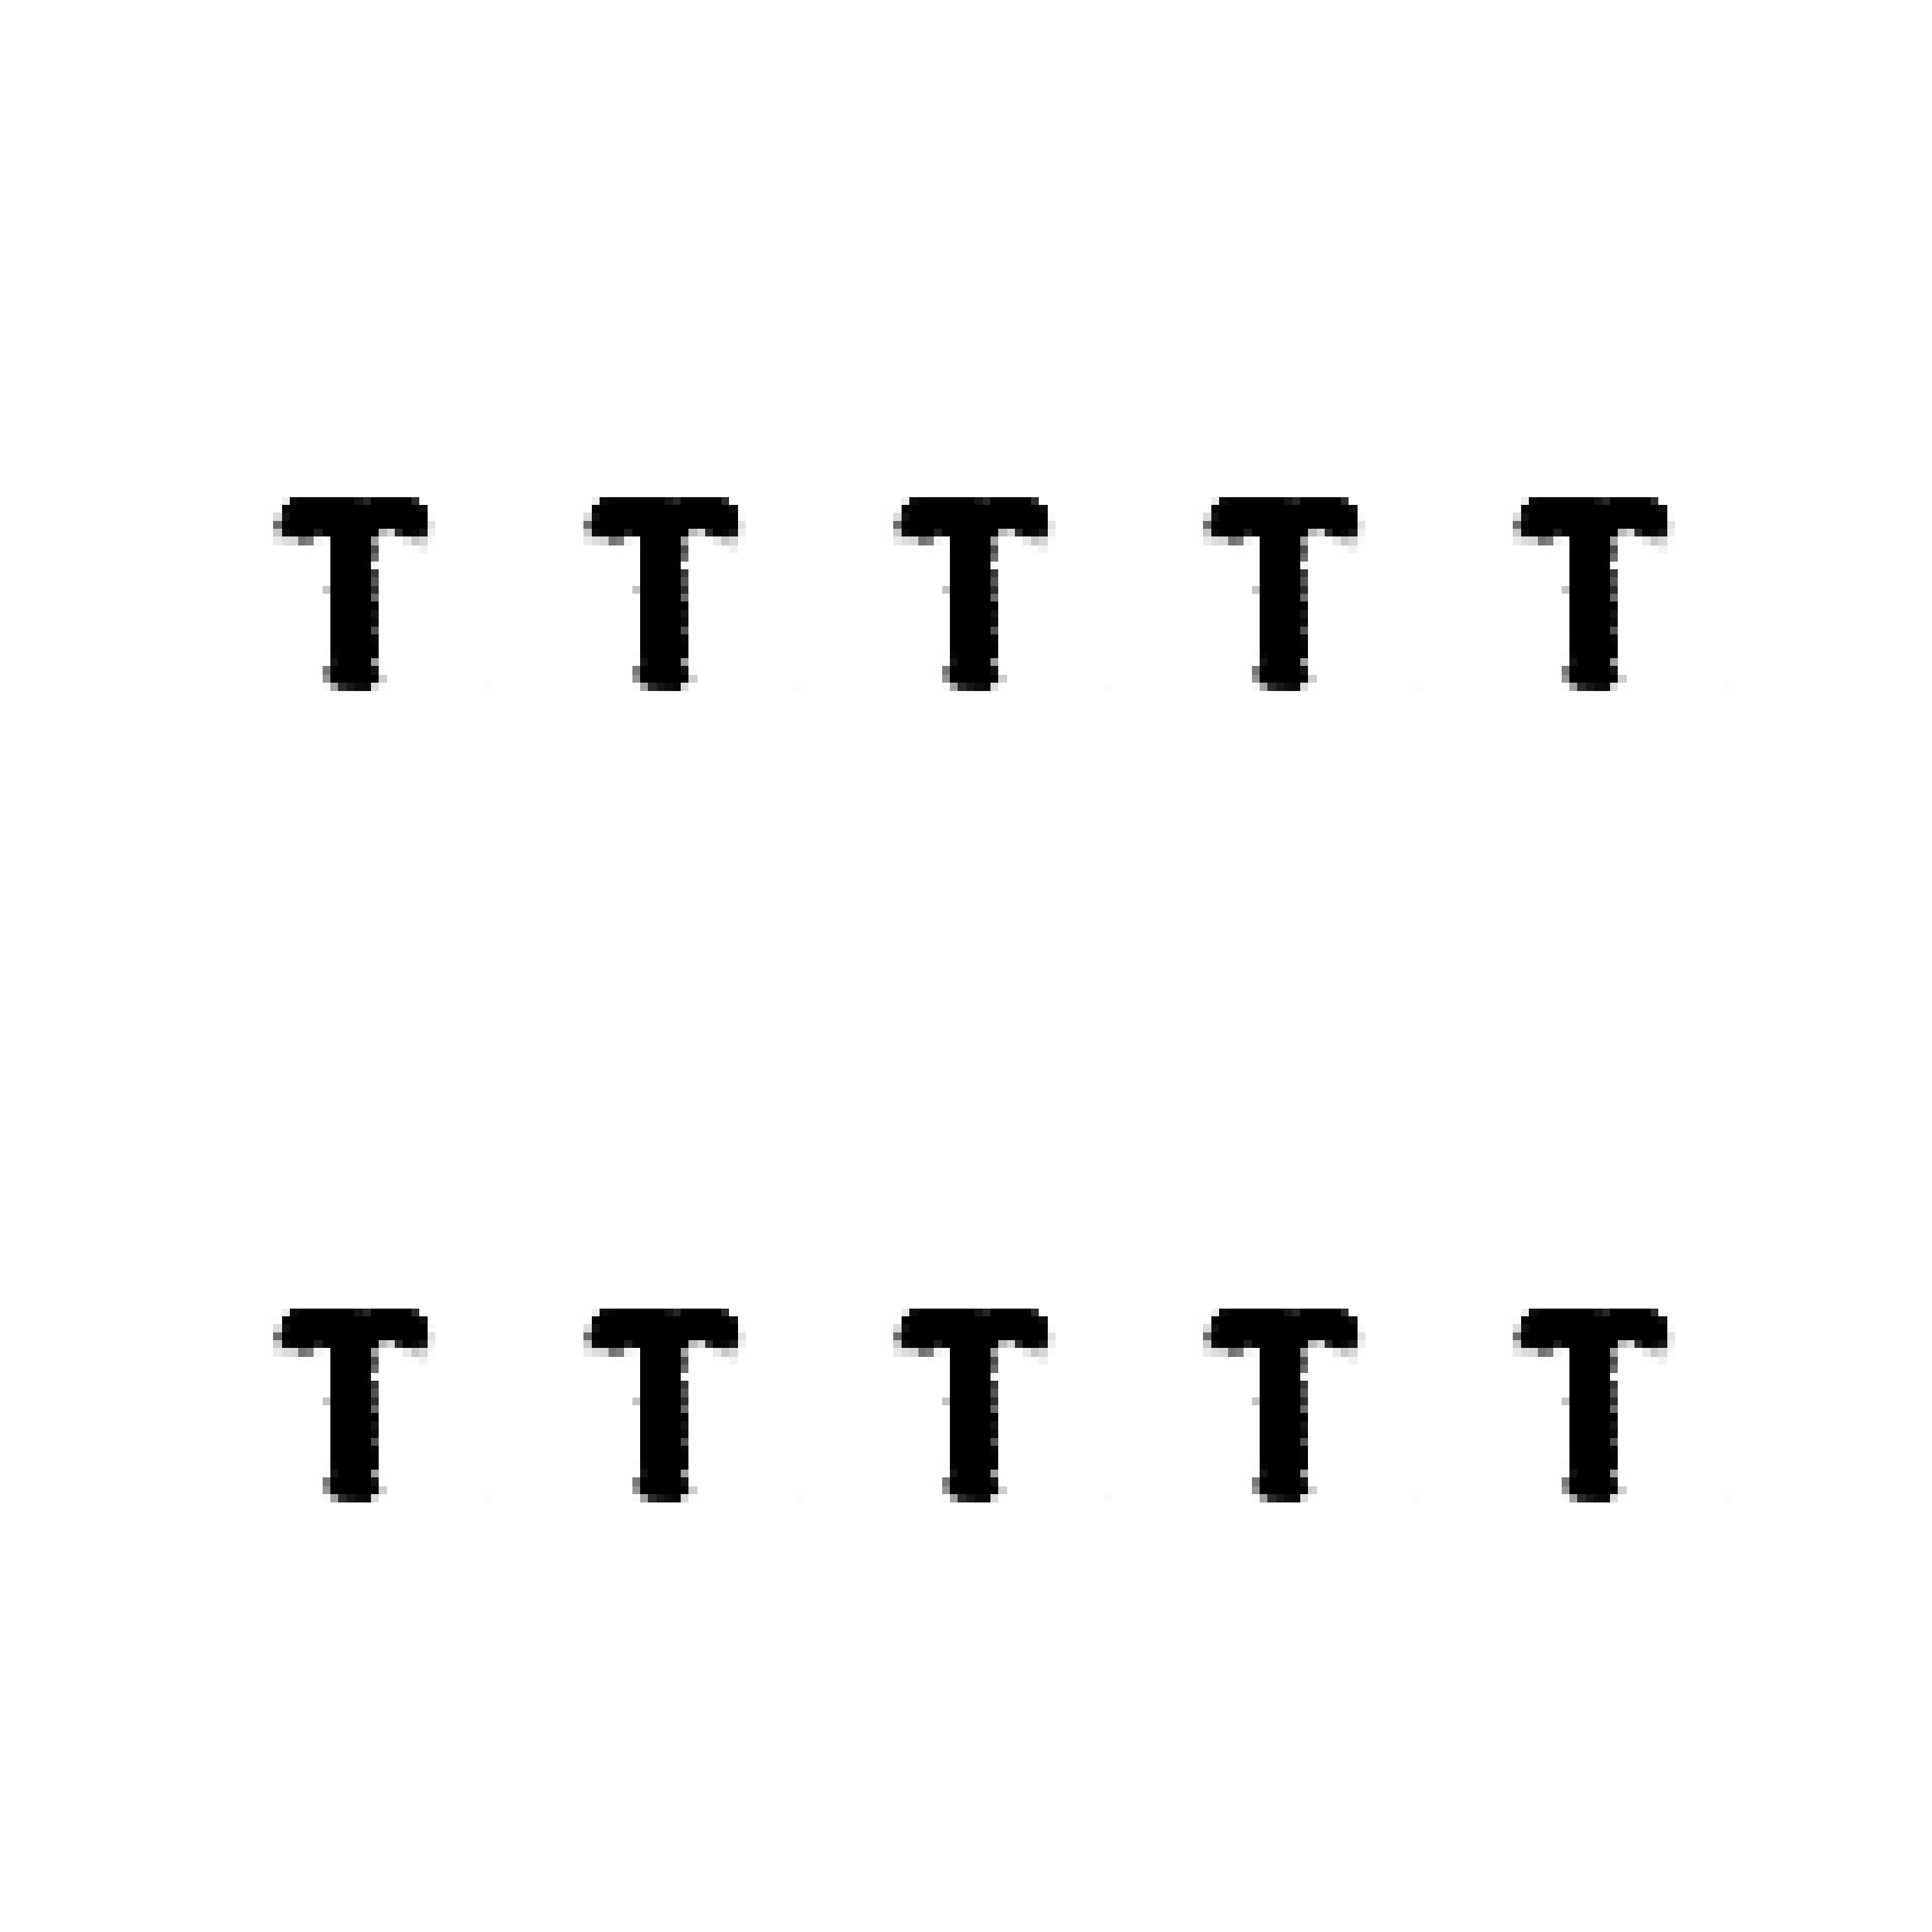
\includegraphics[width=\textwidth , height=\textheight ]{../results/CGAN_Adam/figs/letters/T/95.pdf}}
\end{figure}
\begin{figure}[H]
	\centerline{\includegraphics[width=\textwidth , height=\textheight ]{../results/CGAN_Adam/figs/letters/T/90.pdf}}
\end{figure}

\subsection{حرف \lr{U}}
\begin{figure}[H]
	\centerline{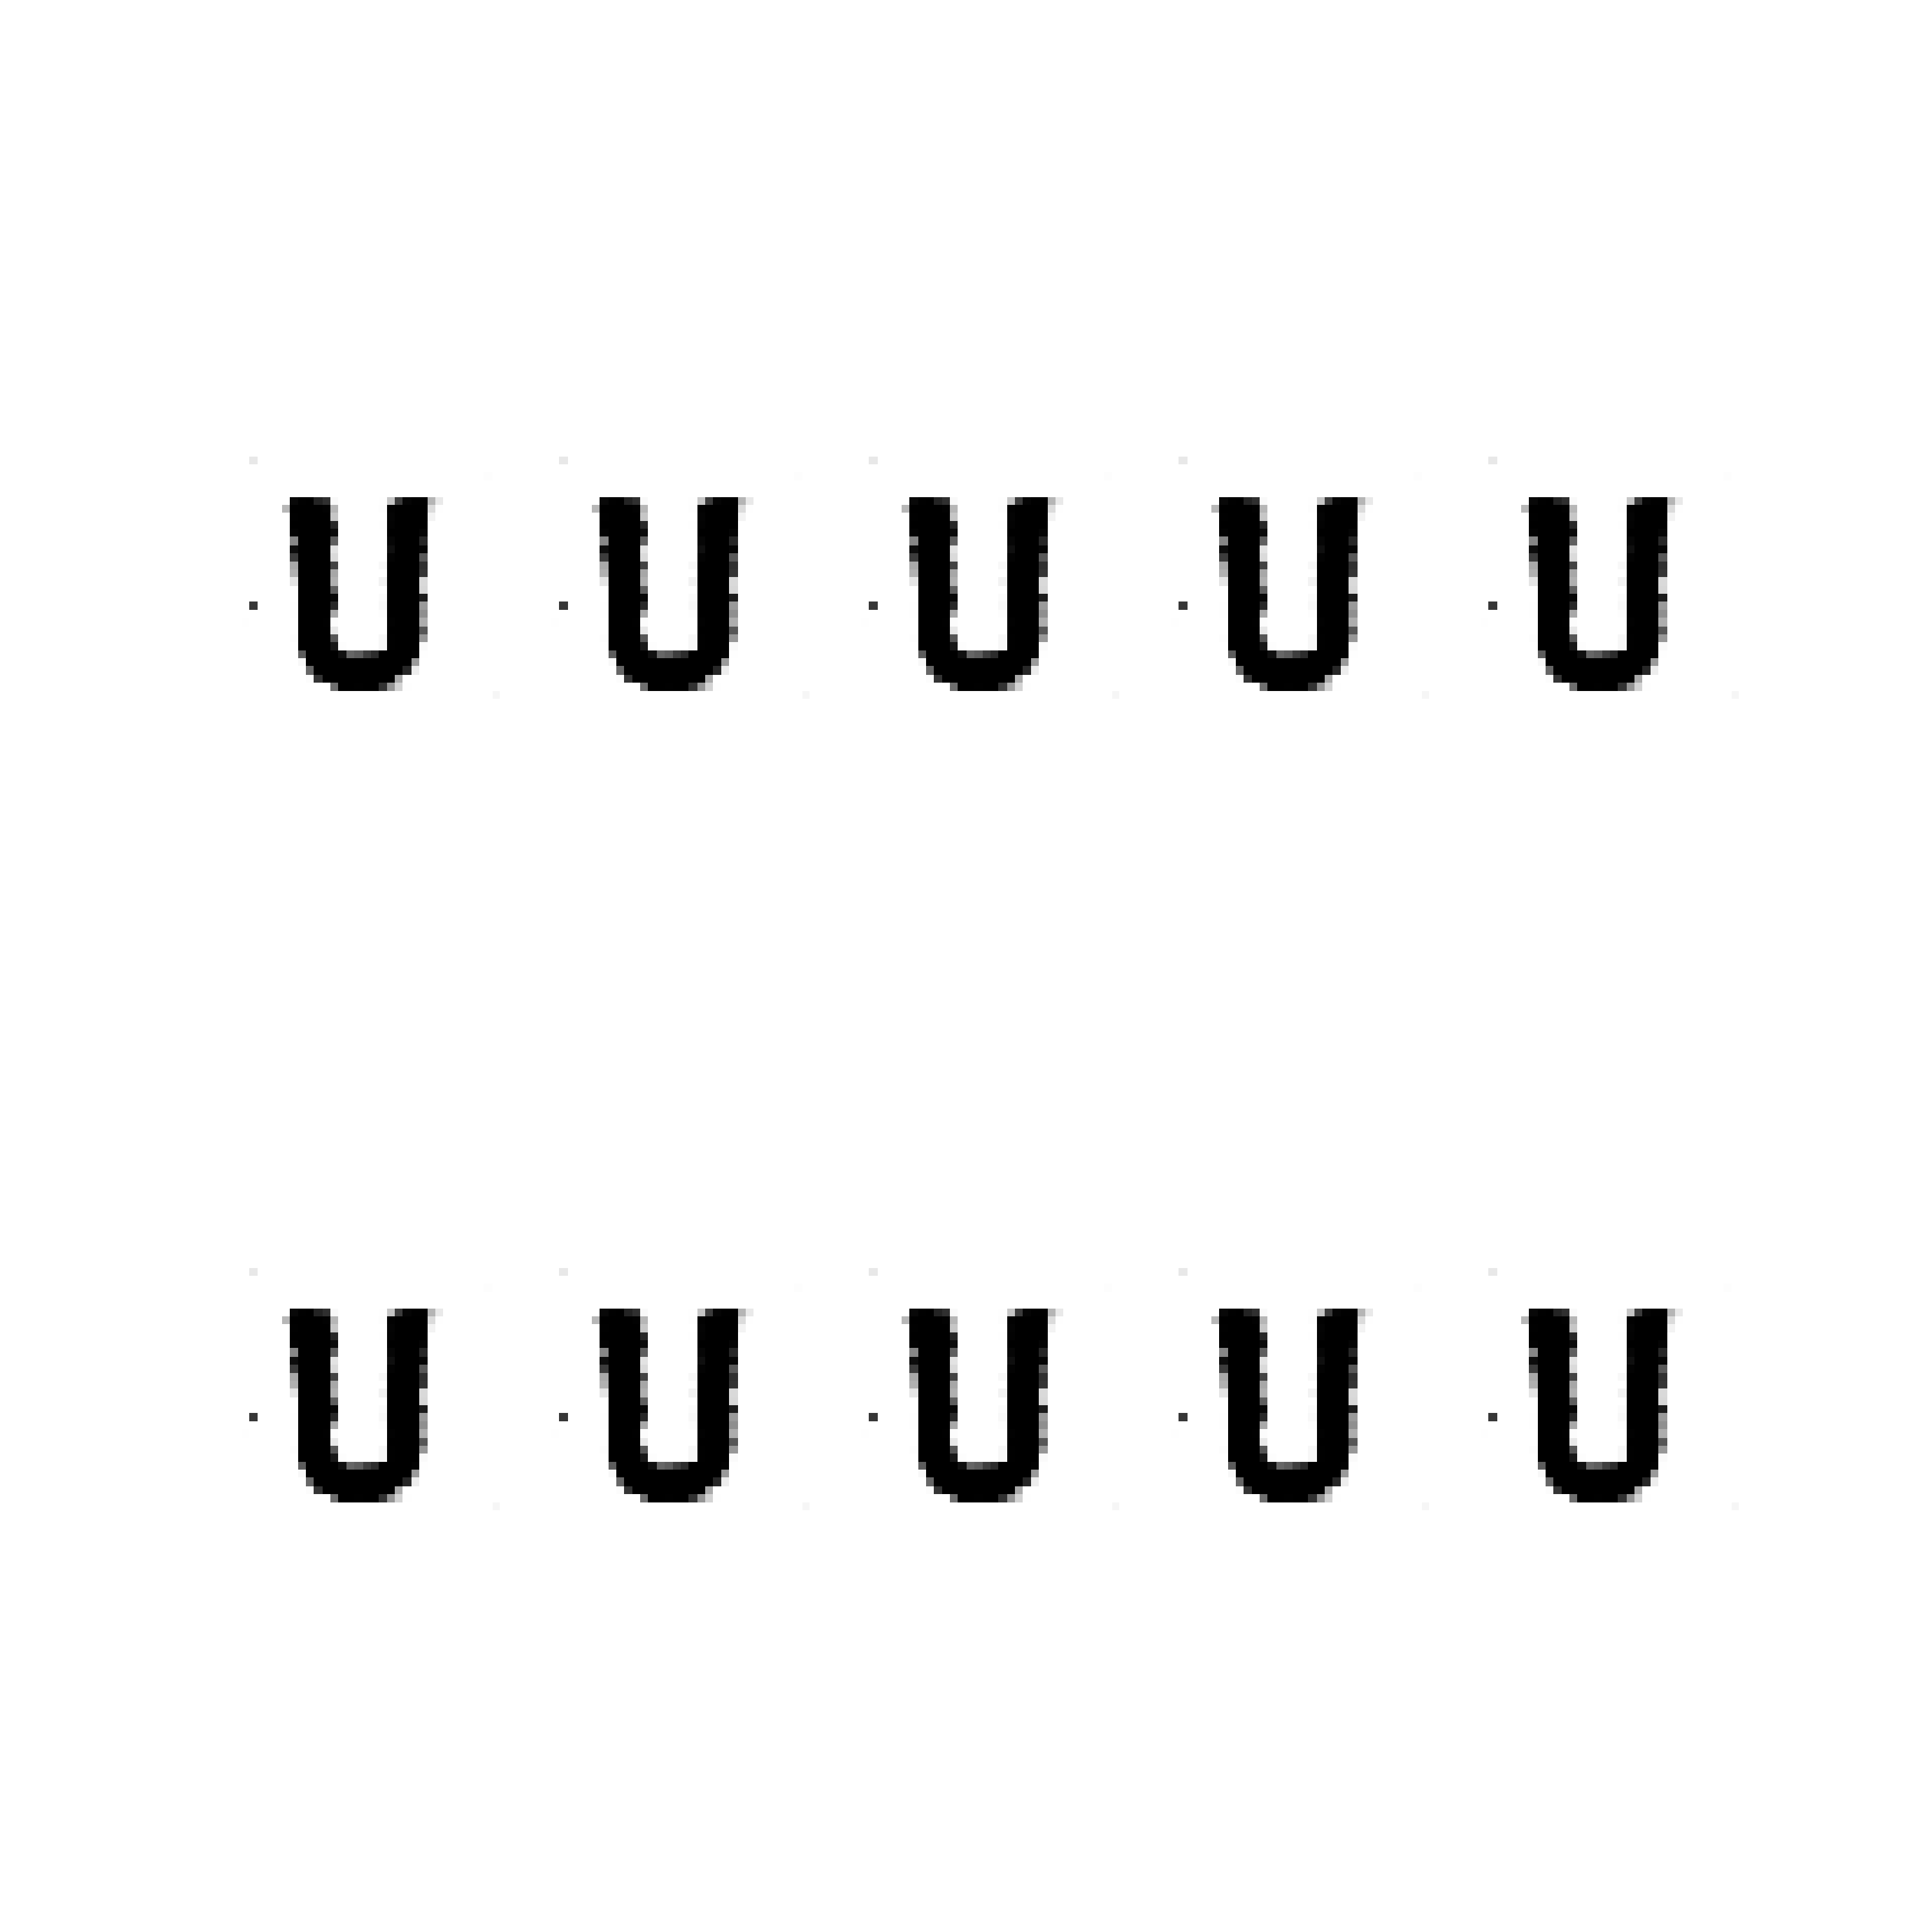
\includegraphics[width=\textwidth , height=\textheight ]{../results/CGAN_Adam/figs/letters/U/95.pdf}}
\end{figure}
\begin{figure}[H]
	\centerline{\includegraphics[width=\textwidth , height=\textheight ]{../results/CGAN_Adam/figs/letters/U/90.pdf}}
\end{figure}

\subsection{حرف \lr{V}}
\begin{figure}[H]
	\centerline{\includegraphics[width=\textwidth , height=\textheight ]{../results/CGAN_Adam/figs/letters/V/95.pdf}}
\end{figure}
\begin{figure}[H]
	\centerline{\includegraphics[width=\textwidth , height=\textheight ]{../results/CGAN_Adam/figs/letters/V/90.pdf}}
\end{figure}

\subsection{حرف \lr{W}}
\begin{figure}[H]
	\centerline{\includegraphics[width=\textwidth , height=\textheight ]{../results/CGAN_Adam/figs/letters/W/95.pdf}}
\end{figure}
\begin{figure}[H]
	\centerline{\includegraphics[width=\textwidth , height=\textheight ]{../results/CGAN_Adam/figs/letters/W/90.pdf}}
\end{figure}

\subsection{حرف \lr{X}}
\begin{figure}[H]
	\centerline{\includegraphics[width=\textwidth , height=\textheight ]{../results/CGAN_Adam/figs/letters/X/95.pdf}}
\end{figure}
\begin{figure}[H]
	\centerline{\includegraphics[width=\textwidth , height=\textheight ]{../results/CGAN_Adam/figs/letters/X/90.pdf}}
\end{figure}

\subsection{حرف \lr{Y}}
\begin{figure}[H]
	\centerline{\includegraphics[width=\textwidth , height=\textheight ]{../results/CGAN_Adam/figs/letters/Y/95.pdf}}
\end{figure}
\begin{figure}[H]
	\centerline{\includegraphics[width=\textwidth , height=\textheight ]{../results/CGAN_Adam/figs/letters/Y/90.pdf}}
\end{figure}

\subsection{حرف \lr{Z}}
\begin{figure}[H]
	\centerline{\includegraphics[width=\textwidth , height=\textheight ]{../results/CGAN_Adam/figs/letters/Z/95.pdf}}
\end{figure}
\begin{figure}[H]
	\centerline{\includegraphics[width=\textwidth , height=\textheight ]{../results/CGAN_Adam/figs/letters/Z/90.pdf}}
\end{figure}




\end{document}